% Use only LaTeX2e, calling the article.cls class and 12-point type.

\documentclass[12pt]{article}

% Users of the {thebibliography} environment or BibTeX should use the
% scicite.sty package, downloadable from *Science* at
% http://www.sciencemag.org/authors/preparing-manuscripts-using-latex 
% This package should properly format in-text
% reference calls and reference-list numbers.

\usepackage{scicite}

\usepackage{times}

% The preamble here sets up a lot of new/revised commands and
% environments.  It's annoying, but please do *not* try to strip these
% out into a separate .sty file (which could lead to the loss of some
% information when we convert the file to other formats).  Instead, keep
% them in the preamble of your main LaTeX source file.


% The following parameters seem to provide a reasonable page setup.

\topmargin 0.0cm
\oddsidemargin 0.2cm
\textwidth 16cm
\textheight 21cm
\footskip 1.0cm

\usepackage{caption}
\usepackage{xcolor, colortbl}
\definecolor{LIGHTGREY}{gray}{0.9}
\usepackage[colorlinks=false]{hyperref}
\usepackage{amssymb,amsfonts,amsmath,amsthm,mathtools}
\usepackage{bm,bbold}
\usepackage{verbatim}
\usepackage{float}
\usepackage{listings, enumerate, enumitem}
\usepackage[export]{adjustbox}
\usepackage{tabu}
\usepackage{longtable}
\tabulinesep=0.6mm
\newcommand\cellwidth{\TX@col@width}
\usepackage{hhline}
\setlength{\arrayrulewidth}{1.2pt}
\usepackage{multicol,multirow,array}
\usepackage{etoolbox}
\AtBeginEnvironment{tabu}{\footnotesize}
\usepackage{booktabs}
\usepackage{makecell}
\usepackage{graphicx}
\usepackage{orcidlink}
\pdfinclusioncopyfonts=1

\renewcommand{\thetable}{S\arabic{table}}
\renewcommand{\thefigure}{S\arabic{figure}}

%The next command sets up an environment for the abstract to your paper.
\newcommand{\UniDimArray}[1]{\bm{#1}}
\newcommand{\der}{\text{d}}
\newcommand{\e}{\text{e}}
\newcommand{\Ne}{N_{\text{e}}}
\newcommand{\proba}{\mathbb{P}}
\newcommand{\pfix}{\proba_{\text{fix}}}
\newcommand{\dn}{d_N}
\newcommand{\ds}{d_S}
\newcommand{\dnds}{\dn / \ds}
\newcommand{\Sphy}{S_{0}}
\newcommand{\SphyDel}{\mathcal{D}_0}
\newcommand{\SphyNeu}{\mathcal{N}_0}
\newcommand{\SphyBen}{\mathcal{B}_0}
\newcommand{\Sphyclass}{x}
\newcommand{\SphyclassAlt}{y}
\newcommand{\given}{\mid}
\newcommand{\Spop}{S}
\newcommand{\SpopDel}{\mathcal{D}}
\newcommand{\SpopNeu}{\mathcal{N}}
\newcommand{\SpopBen}{\mathcal{B}}
\newcommand{\ProbaPopDel}{\proba [ \SpopDel]}
\newcommand{\ProbaPopNeu}{\proba [ \SpopNeu ]}
\newcommand{\ProbaPopBen}{\proba [ \SpopBen ]}
\newcommand{\AdvMean}{\beta_b}
\newcommand{\DelMean}{\beta_d}
\newcommand{\thetaSyn}{\theta_{\text{S}}}


\newenvironment{sciabstract}{%
    \begin{quote} \bf}
    {\end{quote}}


% Include your paper's title here

\title{\textbf{Supplementary materials}\\\vspace*{1cm}Mammalian protein-coding genes exhibit widespread beneficial mutations that are not adaptive}


% Place the author information here.  Please hand-code the contact
% information and notecalls; do *not* use \footnote commands.  Let the
% author contact information appear immediately below the author names
% as shown.  We would also prefer that you don't change the type-size
% settings shown here.

\author
{T. {Latrille}$^{1\dag}$\orcidlink{0000-0002-9643-4668}, J. {Joseph}$^{2\dag}$\orcidlink{0009-0002-1312-9930}, D.~A. {Hartasánchez}$^{1}$\orcidlink{0000-0003-2596-6883}, N. {Salamin}$^{1}$\orcidlink{0000-0002-3963-4954}\\
\\
\normalsize{$^{1}$Department of Computational Biology, Université de Lausanne, Lausanne, Switzerland}\\
\normalsize{$^{2}$Laboratoire de Biométrie et Biologie Evolutive, UMR5558, Université Lyon 1, Villeurbanne, France}\\
\normalsize{$^{\dag}$These authors contributed equally to this work}\\
\normalsize{$^\ast$To whom correspondence should be addressed; E-mail:  \href{mailto:thibault.latrille@ens-lyon.org}{thibault.latrille@ens-lyon.org}.}
}

% Include the date command, but leave its argument blank.

\date{}


%%%%%%%%%%%%%%%%% END OF PREAMBLE %%%%%%%%%%%%%%%%

\begin{document}

% Double-space the manuscript.

    \baselineskip24pt

% Make the title.

    \maketitle

% Place your abstract within the special {sciabstract} environment.

    \begin{sciabstract}
        Mutations can be beneficial by bringing innovation to their bearer, allowing them to adapt to environmental change.
        However, mutations can also be beneficial because they are reverting previous deleterious changes, simply restoring pre-existing functions.
        By integrating phylogenomic and population data in mammals, we estimated the contribution of beneficial back-mutations to molecular evolution, which had remained widely overlooked so far.
        Applying a mutation-selection model, we estimated amino acid fitness landscapes for mammalian protein-coding genes.
        Assuming these fitness landscapes do not change, any beneficial mutation is necessarily a back-mutation.
        We confirmed that these beneficial back-mutations are positively selected in extant populations and demonstrated that a substantial part of ongoing positive selection is not driven by adaptation to environmental change.
    \end{sciabstract}

    \part*{Supplementary materials}
    \tableofcontents
    \clearpage


    \section{Materials \& Methods}
    \label{sec:methods}

    \subsection{Phylogenetic dataset}\label{subsec:phylo-dataset}

    Protein-coding DNA sequence alignments in placental mammals and their corresponding gene trees come from the \href{https://www.orthomam.univ-montp2.fr}{OrthoMaM} database and were processed as in Latrille \textit{et al} (2023)\cite{latrille_genes_2023}.
    OrthoMaM contains a total of $116$ mammalian reference sequences in v10c~\cite{ranwez_orthomam_2007, douzery_orthomam_2014, scornavacca_orthomam_2019}.

    Genes located on the X and Y chromosomes and on the mitochondrial genome were discarded from the analysis because the level of polymorphism –~which is necessary for population-based analyses~– is expected to be different in these three regions compared to the autosomal genome.
    Sequences of species for which we used population-level polymorphism (see section \ref{subsec:polymorphism-dataset}) and their sister species, were removed from the analysis to ensure independence between the data used in the phylogenetic and population scales.
    Sites in the alignment containing more than 10\% of gaps across the species were discarded.
    Altogether, our genome-wide dataset contains $14,509$ protein-coding DNA sequences in $87$ placental mammals.

    \subsection{Selection coefficient ($\Sphy$) in a phylogeny-based method}
    \label{subsec:s-phylogeny-method}

    We analyzed the phylogenetic-level data using mutation-selection models.
    These models assume the protein-coding sequences are at mutation-selection balance under a fixed fitness landscape characterized by a fitness vector over the $20$ amino acids at each site~\cite{yang_mutationselection_2008, halpern_evolutionary_1998, rodrigue_mechanistic_2010}.
    Mathematically, the rate of non-synonymous substitution from codon $a$ to codon $b$ ($q_{a \mapsto b}^{(i)}$) at site $i$ of the sequence is equal to the rate of mutation of the underlying nucleotide change ($\mu_{a \mapsto b}$) multiplied by the scaled probability of mutation fixation ($\proba_{a \mapsto b}^{(i)}$).
    The probability of fixation depends on the difference between the scaled fitness of the amino acid encoded by the mutated codon ($F_b^{(i)}$) and the amino acid encoded by the original codon ($F_a^{(i)}$) at site $i$~\cite{wright_evolution_1931, fisher_genetical_1930}.

    The rate of substitution from codon $a$ to $b$ at a site $i$ is thus:
    \begin{equation}
        \begin{dcases}
            q_{a \mapsto b}^{(i)} & = 0 \text{ if codons $a$ and $b$ are more than one mutation away,} \\
            q_{a \mapsto b}^{(i)} & = \mu_{a \mapsto b} \text{ if codons $a$ and $b$ are synonymous, and}\\
            q_{a \mapsto b}^{(i)} & = \mu_{a \mapsto b} \dfrac{F_b^{(i)} - F_a^{(i)}}{1 - \e^{F_a^{(i)} - F_b^{(i)}}} \text{ if codons $a$ and $b$ are non-synonymous}.
        \end{dcases}
    \end{equation}

    Fitting the mutation-selection model on a multi-species sequence alignment leads to an estimation of the gene-wide $4 \times 4$ nucleotide mutation rate matrix ($\UniDimArray{\mu}$) as well as the $20$ amino-acid fitness landscape ($\UniDimArray{F^{(i)}}$) at each site $i$.
    The selection coefficient for a mutation from codon $a$ to codon $b$ at site $i$ is defined as:
    \begin{equation}
        \Sphy^{(i)} (a \mapsto b) = \Delta F^{(i)} = F^{(i)}_{b} - F^{(i)}_{a}.
    \end{equation}
    In our subsequent derivation the source ($a$) and target ($b$) codons as well as the site ($i$) are implicit and thus never explicitly written.
    We used the Bayesian software \textit{BayesCode} (\url{https://github.com/ThibaultLatrille/bayescode}) to estimate the selection coefficients for each protein-coding gene in the mammalian dataset.
    We ran the Markov chain Monte-Carlo (MCMC) algorithm implemented in BayesCode for $2,000$ generations as described in Latrille \textit{et al} (2023)\cite{latrille_genes_2023}.
    For each gene, after discarding a burn-in period of $1,000$ generations of MCMC, we obtained posterior mean estimates (over the $1,000$ generations left of MCMC) of the mutation rate matrix ($\UniDimArray{\mu}$) as well as the $20$ amino acid fitness landscape ($\UniDimArray{F^{(i)}}$) at each site $i$.

    \subsection{Polymorphism dataset}
    \label{subsec:polymorphism-dataset}

    The genetic variants representing the population level polymorphisms were obtained from the following species and their available datasets: \textit{Equus caballus} (EquCab2 assembly in the EVA study PRJEB9799~\cite{alabri_whole_2020}), \textit{Bos taurus} (UMD3.1 assembly in the NextGen project: \url{https://projects.ensembl.org/nextgen/}), \textit{Ovis aries} (Oar\_v3.1 assembly in the NextGen project), \textit{Capra hircus} (CHIR1 assembly in the NextGen project), converted to ARS1 assembly with dbSNP identifiers~\cite{sherry_dbsnp_2001}), \textit{Chlorocebus sabaeus} (ChlSab1.1 assembly in the EVA project PRJEB22989~\cite{svardal_ancient_2017}), \textit{Homo sapiens} (GRCh38 assembly in the 1000 Genomes Project~\cite{zheng-bradley_alignment_2017}).
    In total, we analyzed 28 populations across the 6 different species with polymorphism data.
    The data was processed as described in Latrille \textit{et al} (2023)\cite{latrille_genes_2023}.

    Only bi-allelic single nucleotide polymorphisms (SNPs) found within a gene were in our polymorphism dataset, while nonsense variants and indels were discarded.
    To construct the dataset, we first recovered the location of each SNP (represented by its chromosome, position, and strand) in the focal species and matched it to its corresponding position in the coding sequence (CDS) using gene annotation files (GTF format) downloaded from Ensembl (\url{ensembl.org}).
    We then verified that the SNP downloaded from Ensembl matched the reference in the CDS in FASTA format.
    Next, the position in the CDS was converted to the corresponding position in the multi-species sequence alignment (containing gaps) from the OrthoMaM database (see section~\ref{subsec:s-phylogeny-method}) for the corresponding gene by doing a global pairwise alignment (Biopython function pairwise2).
    This conversion from genomic position to alignment position was only possible when the assembly used for SNP-calling was the same as the one used in the OrthoMaM alignment, the GTF annotations, and the FASTA sequences.
    SNPs were polarized using the three closest outgroups found in the OrthoMaM alignment with est-usfs v2.04~\cite{keightley_inferring_2018}, and alleles with a probability of being derived lower than 0.99 were discarded.

    \subsection{Mutational opportunities}
    \label{subsec:nunber-of-sites}
    The mutational opportunities of any new mutation refer to its likelihood of falling into a specific category (synonymous, deleterious, nearly-neutral, or beneficial).
    Deriving such opportunities is necessary to estimate the strength of selection exerted at the population scale since different categories might have different mutational opportunities, and thus polymorphism and divergence need to be corrected accordingly (see sections~\ref{subsec:substitution-mapping-in-the-terminal-branch},~\ref{subsec:s-polymorphism-method}, and~\ref{subsec:precisison_recall}).
    To calculate mutational opportunities, we reconstructed the ancestral genome of each of the 28 populations, which differs from the corresponding species' reference genome since it accounts for the variability present in the specific population.
    So, for each population, we used the polarized SNPs to reconstruct the ancestral DNA sequence, containing only substitutions and no segregating polymorphisms.
    If a SNP was still segregating in the population, we used its ancestral version.

    From the reconstructed ancestral genome, all possible mutations were computed, weighted by the instantaneous rate of change between nucleotides obtained from the mutation rate matrix ($\UniDimArray{\mu}$, see section~\ref{subsec:s-phylogeny-method}), summing to $\mu_{\text{tot}}$ across the whole genome, and to $\mu_{\text{syn}}$ when restricted to synonymous mutations.
    Finally, the mutational opportunities for synonymous mutations were computed as the total number of sites across the genome ($L_{\text{tot}}$) weighted by the proportion of synonymous mutations among all possible mutations as:

    \begin{equation}
        L_{\text{syn}} = L_{\text{tot}} \frac{\mu_{\text{syn}}}{\mu_{\text{tot}}}.\label{eq:mutation-opp}
    \end{equation}

    Similarly, for non-synonymous mutations, the total mutation rate for each class of selection $\Sphyclass \in \{\SphyDel, \SphyNeu, \SphyBen \}$, called $\mu\left( \Sphyclass \right)$, was estimated as the sum across all non-synonymous mutations if their selection coefficient at the phylogenetic scale is in the class $\Sphy \in \Sphyclass$.
    Accordingly, the mutational opportunities ($L \left( \Sphyclass \right)$) for each class of selection coefficient ($\Sphyclass$) was finally computed as the total number of sites across the genome ($L_{\text{tot}}$) weighted by the ratio of the aggregated mutations rates falling in the class $\mu\left( \Sphyclass \right)$:
    \begin{equation}
        L \left( \Sphyclass \right) = L_{\text{tot}} \frac{\mu\left( \Sphyclass \right)}{\mu_{\text{tot}}}.
    \end{equation}

    Finally, $\proba [ \Sphyclass ]$ is the probability for a non-synonymous mutation to be in the class $\Sphyclass$, thus computed as:
    \begin{equation}
        \proba[\Sphyclass] = \frac{L\left( \Sphyclass \right)}{\sum_{\SphyclassAlt\in \{\SphyDel, \SphyNeu, \SphyBen \} } L\left(\SphyclassAlt \right)}.
        \label{eq:proba-dfe-mutsel}
    \end{equation}

    \subsection{Substitution mapping and $\dnds$ in the terminal branch}
    \label{subsec:substitution-mapping-in-the-terminal-branch}
    For each gene and each population with polymorphism data available, the genome at the base of the population genealogy was reconstructed (see section~\ref{subsec:nunber-of-sites}).
    We used the ancestral genome reconstructed at the base of the population genealogy and the three closest outgroups found in the OrthoMaM alignment to infer the ancestral protein-coding DNA sequences for each node of the 4-taxa tree by applying the M5 codon model (gamma site rate variation) as implemented in FastML.v3.11~\cite{ashkenazy_fastml_2012}.
    All polarized codon substitutions were then obtained by comparing the ancestral protein-coding DNA sequences before the split from the sister species (closest outgroup) to the genome at the base of the population genealogy.
    We considered \textit{Ceratotherium simum simum} as \textit{Equus caballus'} sister species; \textit{Bison bison bison} as \textit{Bos taurus'} sister species; \textit{Pantholops hodgsonii} as \textit{Ovis aries'} sister species; \textit{Pantholops hodgsonii} as \textit{Capra hircus'} sister species; \textit{Macaca mulatta} as \textit{Chlorocebus sabaeus'} sister species and finally, we considered \textit{Pan troglodytes} as \textit{Homo sapiens'} sister species.
    The selection coefficient ($\Sphy$) of each substitution was then obtained by comparing the difference in amino acid fitnesses for each polarized non-synonymous codon substitution, by referring to the site-specific fitness profile obtained in the phylogeny-based method (see section~\ref{subsec:s-phylogeny-method}).
    Finally, the rate of non-synonymous over synonymous substitutions for a given class of selection coefficient ($\Sphyclass \in \{\SphyDel, \SphyNeu, \SphyBen \}$) was computed as:
    \begin{align}
        \begin{dcases}
            \dn \left( \Sphyclass \right) &= \dfrac{D\left( \Sphyclass \right)}{L \left( \Sphyclass \right)}, \\
            \ds &= \dfrac{D_{\text{syn}}}{L_{\text{syn}}},
        \end{dcases}\label{eq:dnds}
    \end{align}
    where $D \left( \Sphyclass \right) $ was the number of non-synonymous substitutions in class $\Sphyclass$, $D_{\text{syn}}$ was the number of synonymous substitutions across the genome, while $L \left( \Sphyclass \right)$ and $L_{\text{syn}}$ were the numbers of non-synonymous and synonymous mutational opportunities, respectively, as defined in section~\ref{subsec:nunber-of-sites}.
    $\delta(\dnds)$ was computed as the difference between $\dnds$ computed over all substitutions and $\dnds$ when we removed beneficial back-mutations $\dn (\Sphy < 1) / \ds$, normalized by $\dnds$.
    Note that the quantities $\delta(\dnds)$ and $\delta(\dn)$ are equivalent due to the simplification of the factor $\ds$:
    \begin{equation}
        \delta(\dnds) = \dfrac{\dnds - \dn(\Sphy < 1) / \ds}{\dnds} = \dfrac{\dn - \dn(\Sphy < 1)}{\dn} = \delta(\dn).\label{eq:delta-dnds}
    \end{equation}

    \subsection{Scaled selection coefficients ($\Spop$) in a population-based method}
    \label{subsec:s-polymorphism-method}

    To obtain a quantitative estimate of the distribution of selection coefficients for each category of SNPs, we used the polyDFE model~\cite{tataru_inference_2017, tataru_polydfe_2020}.
    This model uses the count of derived alleles to infer the distribution of fitness effects (DFE).
    The probability of sampling an allele at a given frequency (before fixation or extinction) is informative of its scaled selection coefficient at the population scale ($\Spop$).
    Therefore, pooled across many sites, the site-frequency spectrum (SFS) provides information on the underlying $\Spop$ of mutations.
    However, estimating a single $\Spop$ for all sampled mutations is biologically unrealistic, and a DFE of mutations is usually assumed~\cite{eyre-walker_distribution_2006, eyre-walker_estimating_2009}.
    The polyDFE\cite{tataru_inference_2017, tataru_polydfe_2020} software implements a mixture of a $\Gamma$ and exponential distributions to model the DFE of non-synonymous mutations, while synonymous mutations are considered neutral.
    The model estimates the parameters $\DelMean$, $b$, $p_b$ and $\AdvMean$ for non-synonymous mutations as:

    \begin{equation}
        \phi \left( \Spop; \DelMean , b, p_b, \AdvMean \right) =
        \begin{dcases}
            \left( 1 - p_b \right) f_{\Gamma}(-\Spop; -\DelMean, b) & \text{ if $\Spop \leq 0$,} \\
            p_b f_{e}(\Spop; \AdvMean) & \text{ if $\Spop > 0$,} \\
        \end{dcases}
    \end{equation}

    where $\DelMean \leq -1 $ is the estimated mean of the DFE for $\Spop \leq 0$;
    $b \geq 0.2$ is the estimated shape of the $\Gamma$ distribution;
    $0 \leq p_b \leq 1$ is the estimated probability that $\Spop > 0$;
    $\AdvMean \geq 1$ is the estimated mean of the DFE for $\Spop > 0$;
    and $f_{\Gamma}(\Spop; m, b)$ is the density of the $\Gamma$ distribution with mean $m$ and shape $b$, while $f_{e}(\Spop; m)$ is the density of the exponential distribution with mean $m$.

    PolyDFE requires one SFS for non-synonymous mutations and one for synonymous mutations (neutral expectation), as well as the number of sites on which each SFS was sampled.
    For populations containing more than $8$ individuals, the SFS was subsampled down to $16$ chromosomes ($8$ diploid individuals) without replacement (hyper-geometric distribution) to alleviate the effect of different sampling depths in the 28 populations.
    Altogether, for each class of selection ($\Sphyclass \in \{\SphyDel, \SphyNeu, \SphyBen \}$) of non-synonymous SNPs, we aggregated all the SNPs in the selection class $\Sphyclass$ as an SFS.
    The number of sites on which each SFS was sampled is given by $L(\Sphyclass)$ for the non-synonymous SFS and $L_{\text{syn}}$ for the synonymous SFS respectively.
    For each class of selection $\Sphyclass$, once fitted to the data using maximum likelihood with polyDFE, the parameters of the DFE $\left( \DelMean , b, p_b, \AdvMean \right)$ were used to compute $\proba [ \SpopDel \given  \Sphyclass] $, $\proba [ \SpopNeu \given \Sphyclass]$, and $\proba [ \SpopBen \given \Sphyclass]$ as:

    \begin{align}
        \proba [ \SpopDel \given  \Sphyclass] &= \proba [ \Spop < -1 \given \Sphyclass ] = \left( 1 - p_b \right) \int_{1}^{+\infty} f_{\Gamma}(\Spop; -\DelMean, b) \der \Spop, \label{eq:polyProbaDel} \\
        \proba [ \SpopNeu \given \Sphyclass] &= \proba [ -1 < \Spop < 1 \given \Sphyclass ] = p_b \int_{0}^{1} f_{e}(\Spop; \AdvMean) \der \Spop + \left( 1 - p_b \right) \int_{0}^{1} f_{\Gamma}(\Spop; -\DelMean, b) \der \Spop, \\
        \proba [ \SpopBen \given \Sphyclass] &= \proba [ \Spop > 1 \given \Sphyclass] = p_b \int_{1}^{+\infty} f_{e}(\Spop; \AdvMean) \der \Spop. \label{eq:polyProbaAdv}
    \end{align}

    \subsection{\textit{Precision} and \textit{recall}}
    \label{subsec:precisison_recall}
    For readability, we give here \textit{precision} and \textit{recall} for beneficial mutations ($\SphyBen$ and $\SpopBen$), but it can be obtained using the same derivation for the deleterious mutations ($\SphyDel$ and $\SpopDel$) and nearly-neutral mutations ($\SphyNeu$ and $\SpopNeu$).

    \textit{Precision} is the proportion of mutations correctly predicted as beneficial ($\proba [ \SpopBen \cap  \SphyBen]$) out of all predicted as beneficial back-mutations ($\proba [ \SphyBen]$), which can be written as a conditional probability:

    \begin{equation}
        \frac{\proba [ \SpopBen  \cap  \SphyBen]}{\proba [ \SphyBen]} = \proba [ \SpopBen  \given  \SphyBen].
        \label{eq:precision}
    \end{equation}
    Namely, \textit{precision} corresponds to the probability for a back-mutation ($\SphyBen$) to be effectively beneficial at the population level ($\SpopBen$).
    This probability, computed from eq.~\ref{eq:polyProbaAdv}, is obtained by restricting our analysis to SNPs that are predicted to be beneficial back-mutations (yellow fill for the category $\SphyBen$ in fig.~3D).

    \textit{Recall} is the proportion of mutations correctly predicted as beneficial ($\proba [ \SpopBen \cap  \SphyBen]$) out of all beneficial mutations ($\proba [ \SpopBen]$), which can be written as a conditional probability:
    \begin{equation}
        \frac{\proba [ \SpopBen \cap  \SphyBen]}{\proba [ \SpopBen]} = \proba [ \SphyBen  \given \SpopBen ].
    \end{equation}
    Namely, \textit{recall} corresponds to the probability for a beneficial mutation at the population level ($\SpopBen$) to be a beneficial back-mutation ($\SphyBen$).
    Using Bayes theorem, \textit{recall} can be re-written as:
    \begin{equation}
        \proba [\SphyBen \given \SpopBen] = \frac{\proba [\SpopBen \given \SphyBen] \times \proba[\SphyBen]}{\ProbaPopBen},
        \label{eq:bayes}
    \end{equation}

    where $\proba [\SpopBen \given \SphyBen]$ and $\proba [ \SphyBen ]$ can be calculated using equations~\ref{eq:precision} and~\ref{eq:proba-dfe-mutsel}, respectively, and $\proba [ \SpopBen ]$ is the probability of a mutation to be beneficial at the level of the population, which can be computed from the law of total probabilities as:

    \begin{equation}
        \proba [ \SpopBen ] = \sum_{\Sphyclass \in \{\SphyDel, \SphyNeu, \SphyBen \} }\proba [\SpopBen \given \Sphyclass ] \times \proba [\Sphyclass ].
        \label{eq:total_proba}
    \end{equation}

\section{Beneficial mutations in the terminal lineages and populations}\label{sec:beneficial-mutations}

    \subsection{Mutation-selection codon models}
    \label{sec:site-specific-mutation-selection-codon-models}
    In \textit{BayesCode} (\url{https://github.com/ThibaultLatrille/bayescode}), we ran the mutation-selection codon models \textit{mutselomega} for 2000 points of MCMC with the options:
    \begin{scriptsize}
        \begin{verbatim}
 mutselomega ---omegashift 0.0 --ncat 30 -a my_alignment.phy -t my_tree.newick -u 2000 my_genename
        \end{verbatim}
    \end{scriptsize}
    The collection of site-specific fitness profiles ($\UniDimArray{F^{(i)}}, \forall i$) are then obtained by running \textit{readmutselomega}, reading 1000 points of MCMC (first 1000 are considered as burn-in) with the options:
    \begin{scriptsize}
        \begin{verbatim}
 readmutselomega --every 1 --until 2000 --burnin 1000 --ss my_genename
        \end{verbatim}
    \end{scriptsize}
    The gene-specific $4 \times 4$ nucleotide mutation rate matrix ($\UniDimArray{\mu}$) is also obtained by running \textit{readmutselomega}, reading 1000 points of MCMC (first 1000 are considered as burn-in) with the options:
    \begin{scriptsize}
        \begin{verbatim}
 readmutselomega --every 1 --until 2000 --burnin 1000 --nuc my_genename
        \end{verbatim}
    \end{scriptsize}

    \subsection{Summary tables}\label{subsec:summary-table-mutsel}

    \subsubsection{$\dnds$ for deleterious ($\SphyDel$), nearly-neutral ($\SphyNeu$) and beneficial back-mutations ($\SphyBen$)}
    \begin{center}
        \captionof{table}{$\dnds$ for deleterious ($\SphyDel$), nearly-neutral ($\SphyNeu$) and beneficial back-mutations ($\SphyBen$).}
        \scriptsize
        \begin{longtable*}{|l|l|r|r|r|r|r|r|}
            \toprule
            Population &             Species & Watterson's $\thetaSyn$  & $\proba_{div}[ \SphyBen ]$ & $\dnds $ & $\dn ( \SphyDel ) / \ds$ & $\dn ( \SphyNeu ) / \ds$ & $\dn ( \SphyBen ) / \ds$ \\
            \midrule
            \endhead
            \midrule
            \multicolumn{8}{r}{{Continued on next page}} \\
            \midrule
            \endfoot

            \bottomrule
            \endlastfoot
            \rowcolor{LIGHTGREY} Equus c. &      Equus caballus &               $ 0.002$ &                    $ 0.118$ &  $ 0.147$ &            $ 0.075$ &                $ 0.823$ &           $ 1.203$ \\
            Iran &          Bos taurus &               $ 0.002$ &                    $ 0.123$ &  $ 0.131$ &            $ 0.074$ &                $ 0.627$ &           $ 1.206$ \\
            Uganda &          Bos taurus &               $ 0.005$ &                    $ 0.125$ &  $ 0.134$ &            $ 0.075$ &                $ 0.637$ &           $ 1.252$ \\
            \rowcolor{LIGHTGREY} Australia &        Capra hircus &               $ 0.003$ &                    $ 0.121$ &  $ 0.125$ &            $ 0.068$ &                $ 0.629$ &           $ 1.099$ \\
            \rowcolor{LIGHTGREY} France &        Capra hircus &               $ 0.004$ &                    $ 0.120$ &  $ 0.126$ &            $ 0.068$ &                $ 0.633$ &           $ 1.102$ \\
            \rowcolor{LIGHTGREY} Iran (C. aegagrus) &        Capra hircus &               $ 0.004$ &                    $ 0.120$ &  $ 0.125$ &            $ 0.068$ &                $ 0.630$ &           $ 1.100$ \\
            \rowcolor{LIGHTGREY} Iran &        Capra hircus &               $ 0.004$ &                    $ 0.121$ &  $ 0.125$ &            $ 0.067$ &                $ 0.630$ &           $ 1.108$ \\
            \rowcolor{LIGHTGREY} Italy &        Capra hircus &               $ 0.004$ &                    $ 0.120$ &  $ 0.126$ &            $ 0.068$ &                $ 0.634$ &           $ 1.102$ \\
            \rowcolor{LIGHTGREY} Morocco &        Capra hircus &               $ 0.004$ &                    $ 0.122$ &  $ 0.125$ &            $ 0.067$ &                $ 0.631$ &           $ 1.112$ \\
            Iran &          Ovis aries &               $ 0.007$ &                    $ 0.109$ &  $ 0.146$ &            $ 0.091$ &                $ 0.616$ &           $ 1.148$ \\
            Iran (O. orientalis) &          Ovis aries &               $ 0.009$ &                    $ 0.108$ &  $ 0.148$ &            $ 0.093$ &                $ 0.617$ &           $ 1.145$ \\
            Iran (O. vignei) &          Ovis aries &               $ 0.007$ &                    $ 0.109$ &  $ 0.146$ &            $ 0.091$ &                $ 0.617$ &           $ 1.134$ \\
            Various &          Ovis aries &               $ 0.008$ &                    $ 0.107$ &  $ 0.148$ &            $ 0.093$ &                $ 0.617$ &           $ 1.134$ \\
            Morocco &          Ovis aries &               $ 0.008$ &                    $ 0.108$ &  $ 0.148$ &            $ 0.093$ &                $ 0.619$ &           $ 1.149$ \\
            \rowcolor{LIGHTGREY} Barbados & Chlorocebus sabaeus &               $ 0.004$ &                    $ 0.122$ &  $ 0.133$ &            $ 0.071$ &                $ 0.696$ &           $ 1.397$ \\
            \rowcolor{LIGHTGREY} Central Afr. Rep. & Chlorocebus sabaeus &               $ 0.006$ &                    $ 0.124$ &  $ 0.134$ &            $ 0.071$ &                $ 0.701$ &           $ 1.431$ \\
            \rowcolor{LIGHTGREY} Ethiopia & Chlorocebus sabaeus &               $ 0.005$ &                    $ 0.124$ &  $ 0.134$ &            $ 0.071$ &                $ 0.699$ &           $ 1.422$ \\
            \rowcolor{LIGHTGREY} Gambia & Chlorocebus sabaeus &               $ 0.005$ &                    $ 0.123$ &  $ 0.134$ &            $ 0.071$ &                $ 0.703$ &           $ 1.411$ \\
            \rowcolor{LIGHTGREY} Kenya & Chlorocebus sabaeus &               $ 0.005$ &                    $ 0.123$ &  $ 0.134$ &            $ 0.071$ &                $ 0.699$ &           $ 1.419$ \\
            \rowcolor{LIGHTGREY} Nevis & Chlorocebus sabaeus &               $ 0.003$ &                    $ 0.123$ &  $ 0.133$ &            $ 0.071$ &                $ 0.699$ &           $ 1.407$ \\
            \rowcolor{LIGHTGREY} South Africa  & Chlorocebus sabaeus &               $ 0.006$ &                    $ 0.125$ &  $ 0.134$ &            $ 0.070$ &                $ 0.704$ &           $ 1.447$ \\
            \rowcolor{LIGHTGREY} Saint Kitts & Chlorocebus sabaeus &               $ 0.004$ &                    $ 0.123$ &  $ 0.133$ &            $ 0.070$ &                $ 0.699$ &           $ 1.413$ \\
            \rowcolor{LIGHTGREY} Zambia & Chlorocebus sabaeus &               $ 0.006$ &                    $ 0.123$ &  $ 0.134$ &            $ 0.071$ &                $ 0.699$ &           $ 1.410$ \\
            African &        Homo sapiens &               $ 0.002$ &                    $ 0.099$ &  $ 0.192$ &            $ 0.118$ &                $ 0.865$ &           $ 1.609$ \\
            Admixed American &        Homo sapiens &               $ 0.002$ &                    $ 0.099$ &  $ 0.192$ &            $ 0.118$ &                $ 0.865$ &           $ 1.607$ \\
            East Asian &        Homo sapiens &               $ 0.002$ &                    $ 0.098$ &  $ 0.192$ &            $ 0.118$ &                $ 0.869$ &           $ 1.607$ \\
            European &        Homo sapiens &               $ 0.002$ &                    $ 0.098$ &  $ 0.192$ &            $ 0.118$ &                $ 0.865$ &           $ 1.598$ \\
            South Asian &        Homo sapiens &               $ 0.002$ &                    $ 0.099$ &  $ 0.192$ &            $ 0.118$ &                $ 0.867$ &           $ 1.610$ \\
        \end{longtable*}
    \end{center}
    \begin{itemize}
        \item Watterson's $\thetaSyn$ is the observed genetic diversity calculated for synonymous changes.
        \item $\proba_{div}[\SphyBen]$ is the proportion of substitutions in the terminal branch that are $\SphyBen$.
        \item $\dn(\SphyDel) / \ds$ (eq.~\ref{eq:dnds}) is the ratio of non-synonymous over synonymous substitutions, when restricted to non-synonymous substitutions in the terminal branch that are $\SphyDel$.
        \item $\dn(\SphyNeu) / \ds$ (eq.~\ref{eq:dnds}) is the ratio of non-synonymous over synonymous substitutions, when restricted to non-synonymous substitutions in the terminal branch that are $\SphyNeu$.
        \item $\dn(\SphyBen) / \ds$ (eq.~\ref{eq:dnds}) is the ratio of non-synonymous over synonymous substitutions, when restricted to non-synonymous substitutions in the terminal branch that are $\SphyBen$.
    \end{itemize}

    \newpage

    \subsubsection{$\dnds$ over-estimation due to beneficial back-mutations}
    \begin{center}
        \captionof{table}{$\dnds$ over-estimation due to beneficial back-mutations.}
        \scriptsize
        \begin{longtable*}{|l|l|r|r|r|r|r|}
            \toprule
            Population & Species & Watterson's $\thetaSyn$ & $\proba_{div}[\Sphy > 1]$ & $\dnds $ & $\dn(\Sphy < 1) / \ds$ & $\delta(\dnds )$ \\
            \midrule
            \endhead
            \midrule
            \multicolumn{7}{r}{{Continued on next page}} \\
            \midrule
            \endfoot

            \bottomrule
            \endlastfoot
            \rowcolor{LIGHTGREY} Equus c. &      Equus caballus &               $ 0.002$ &                    $ 0.118$ &  $ 0.147$ &           $ 0.131$ &     $  10.5$ \\
            Iran &          Bos taurus &               $ 0.002$ &                    $ 0.123$ &  $ 0.131$ &           $ 0.117$ &     $  11.1$ \\
            Uganda &          Bos taurus &               $ 0.005$ &                    $ 0.125$ &  $ 0.134$ &           $ 0.118$ &     $  11.3$ \\
            \rowcolor{LIGHTGREY} Australia &        Capra hircus &               $ 0.003$ &                    $ 0.121$ &  $ 0.125$ &           $ 0.111$ &     $  10.8$ \\
            \rowcolor{LIGHTGREY} France &        Capra hircus &               $ 0.004$ &                    $ 0.120$ &  $ 0.126$ &           $ 0.112$ &     $  10.8$ \\
            \rowcolor{LIGHTGREY} Iran (C. aegagrus) &        Capra hircus &               $ 0.004$ &                    $ 0.120$ &  $ 0.125$ &           $ 0.111$ &     $  10.8$ \\
            \rowcolor{LIGHTGREY} Iran &        Capra hircus &               $ 0.004$ &                    $ 0.121$ &  $ 0.125$ &           $ 0.111$ &     $  10.9$ \\
            \rowcolor{LIGHTGREY} Italy &        Capra hircus &               $ 0.004$ &                    $ 0.120$ &  $ 0.126$ &           $ 0.112$ &     $  10.8$ \\
            \rowcolor{LIGHTGREY} Morocco &        Capra hircus &               $ 0.004$ &                    $ 0.122$ &  $ 0.125$ &           $ 0.111$ &     $  11.0$ \\
            Iran &          Ovis aries &               $ 0.007$ &                    $ 0.109$ &  $ 0.146$ &           $ 0.132$ &     $ 9.671$ \\
            Iran (O. orientalis) &          Ovis aries &               $ 0.009$ &                    $ 0.108$ &  $ 0.148$ &           $ 0.134$ &     $ 9.516$ \\
            Iran (O. vignei) &          Ovis aries &               $ 0.007$ &                    $ 0.109$ &  $ 0.146$ &           $ 0.132$ &     $ 9.598$ \\
            Various &          Ovis aries &               $ 0.008$ &                    $ 0.107$ &  $ 0.148$ &           $ 0.134$ &     $ 9.439$ \\
            Morocco &          Ovis aries &               $ 0.008$ &                    $ 0.108$ &  $ 0.148$ &           $ 0.134$ &     $ 9.582$ \\
            \rowcolor{LIGHTGREY} Barbados & Chlorocebus sabaeus &               $ 0.004$ &                    $ 0.122$ &  $ 0.133$ &           $ 0.118$ &     $  11.2$ \\
            \rowcolor{LIGHTGREY} Central Afr. Rep. & Chlorocebus sabaeus &               $ 0.006$ &                    $ 0.124$ &  $ 0.134$ &           $ 0.119$ &     $  11.3$ \\
            \rowcolor{LIGHTGREY} Ethiopia & Chlorocebus sabaeus &               $ 0.005$ &                    $ 0.124$ &  $ 0.134$ &           $ 0.118$ &     $  11.3$ \\
            \rowcolor{LIGHTGREY} Gambia & Chlorocebus sabaeus &               $ 0.005$ &                    $ 0.123$ &  $ 0.134$ &           $ 0.119$ &     $  11.2$ \\
            \rowcolor{LIGHTGREY} Kenya & Chlorocebus sabaeus &               $ 0.005$ &                    $ 0.123$ &  $ 0.134$ &           $ 0.119$ &     $  11.3$ \\
            \rowcolor{LIGHTGREY} Nevis & Chlorocebus sabaeus &               $ 0.003$ &                    $ 0.123$ &  $ 0.133$ &           $ 0.118$ &     $  11.3$ \\
            \rowcolor{LIGHTGREY} South Africa  & Chlorocebus sabaeus &               $ 0.006$ &                    $ 0.125$ &  $ 0.134$ &           $ 0.118$ &     $  11.5$ \\
            \rowcolor{LIGHTGREY} Saint Kitts & Chlorocebus sabaeus &               $ 0.004$ &                    $ 0.123$ &  $ 0.133$ &           $ 0.118$ &     $  11.3$ \\
            \rowcolor{LIGHTGREY} Zambia & Chlorocebus sabaeus &               $ 0.006$ &                    $ 0.123$ &  $ 0.134$ &           $ 0.119$ &     $  11.2$ \\
            African &        Homo sapiens &               $ 0.002$ &                    $ 0.099$ &  $ 0.192$ &           $ 0.175$ &     $ 8.799$ \\
            Admixed American &        Homo sapiens &               $ 0.002$ &                    $ 0.099$ &  $ 0.192$ &           $ 0.175$ &     $ 8.780$ \\
            East Asian &        Homo sapiens &               $ 0.002$ &                    $ 0.098$ &  $ 0.192$ &           $ 0.175$ &     $ 8.768$ \\
            European &        Homo sapiens &               $ 0.002$ &                    $ 0.098$ &  $ 0.192$ &           $ 0.175$ &     $ 8.728$ \\
            South Asian &        Homo sapiens &               $ 0.002$ &                    $ 0.099$ &  $ 0.192$ &           $ 0.175$ &     $ 8.788$ \\
        \end{longtable*}
    \end{center}
    \begin{itemize}
        \item Watterson's $\thetaSyn$ is the observed genetic diversity calculated for synonymous changes.
        \item $\proba_{div}[\SphyBen]$ is the proportion of substitutions in the terminal branch that are $\SphyBen$.
        \item $\dnds$ (eq.~\ref{eq:dnds}) is the ratio of non-synonymous over synonymous substitutions estimated for all the non-synonymous substitutions in the terminal branch.
        \item $\dn(\Sphy < 1) / \ds$ (eq.~\ref{eq:dnds}) is the ratio of non-synonymous over synonymous substitutions, when restricted to non-synonymous substitutions in the terminal branch that are not $\SphyBen$.
        This is the estimated divergence when we removed beneficial back-mutations.
        \item $\delta(\dnds)$ (eq.~7) is the fraction of the divergence ($\dnds$) that is over-estimated, $\dnds$ is compared to the estimated divergence when we removed beneficial back-mutations $\dn(\Sphy < 1) / \ds$.
    \end{itemize}
    We estimated that between 9 and 11\% of $\dnds$ is over-estimated, corresponding to beneficial back-mutation inflating the $\dnds$ statistic.

    \newpage

    \subsubsection{Probabilities of beneficial back-mutations}
    \begin{center}
        \captionof{table}{Probability of beneficial back-mutations among all beneficial ones.}
        \scriptsize
        \begin{longtable*}{|l|l|r|r|r|r|r|r|}
            \toprule
            Population & Species & Watterson's $\thetaSyn$ & $\proba[\SphyBen]$ & $\proba [ \SpopBen ]$ & $\frac{\proba[\SphyBen]}{\proba[ \SpopBen ]}$ & $\proba [ \SpopBen \given \SphyBen]$ & $\proba[\SphyBen\given \SpopBen ]$ \\
            \midrule
            \endhead
            \midrule
            \multicolumn{8}{r}{{Continued on next page}} \\
            \midrule
            \endfoot

            \bottomrule
            \endlastfoot
            \rowcolor{LIGHTGREY} Equus c. &      Equus caballus &               $ 0.002$ &              $ 0.014$ &              $ 0.010$ &                                          $ 1.395$ &                         $ 0.580$ &                      $ 0.809$ \\
            Iran &          Bos taurus &               $ 0.002$ &              $ 0.013$ &              $ 0.041$ &                                          $ 0.323$ &                         $ 0.857$ &                      $ 0.277$ \\
            Uganda &          Bos taurus &               $ 0.005$ &              $ 0.013$ &              $ 0.013$ &                                          $ 0.991$ &                         $ 0.488$ &                      $ 0.483$ \\
            \rowcolor{LIGHTGREY} Australia &        Capra hircus &               $ 0.003$ &              $ 0.014$ &              $ 0.026$ &                                          $ 0.532$ &                         $ 0.368$ &                      $ 0.196$ \\
            \rowcolor{LIGHTGREY} France &        Capra hircus &               $ 0.004$ &              $ 0.014$ &              $ 0.024$ &                                          $ 0.572$ &                         $ 0.368$ &                      $ 0.211$ \\
            \rowcolor{LIGHTGREY} Iran (C. aegagrus) &        Capra hircus &               $ 0.004$ &              $ 0.014$ &              $ 0.026$ &                                          $ 0.516$ &                         $ 0.221$ &                      $ 0.114$ \\
            \rowcolor{LIGHTGREY} Iran &        Capra hircus &               $ 0.004$ &              $ 0.014$ &              $ 0.024$ &                                          $ 0.573$ &                         $ 0.368$ &                      $ 0.211$ \\
            \rowcolor{LIGHTGREY} Italy &        Capra hircus &               $ 0.004$ &              $ 0.014$ &              $ 0.017$ &                                          $ 0.814$ &                         $ 0.270$ &                      $ 0.220$ \\
            \rowcolor{LIGHTGREY} Morocco &        Capra hircus &               $ 0.004$ &              $ 0.014$ &              $ 0.018$ &                                          $ 0.751$ &                         $ 0.368$ &                      $ 0.276$ \\
            Iran &          Ovis aries &               $ 0.007$ &              $ 0.014$ &              $ 0.006$ &                                          $ 2.321$ &                         $ 0.169$ &                      $ 0.392$ \\
            Iran (O. orientalis) &          Ovis aries &               $ 0.009$ &              $ 0.014$ &              $ 0.012$ &                                          $ 1.178$ &                         $ 0.153$ &                      $ 0.180$ \\
            Iran (O. vignei) &          Ovis aries &               $ 0.007$ &              $ 0.014$ &              $ 0.020$ &                                          $ 0.683$ &                         $ 0.195$ &                      $ 0.133$ \\
            Various &          Ovis aries &               $ 0.008$ &              $ 0.014$ &              $ 0.012$ &                                          $ 1.201$ &                         $ 0.190$ &                      $ 0.228$ \\
            Morocco &          Ovis aries &               $ 0.008$ &              $ 0.014$ &              $ 0.005$ &                                          $ 2.589$ &                         $ 0.136$ &                      $ 0.353$ \\
            \rowcolor{LIGHTGREY} Barbados & Chlorocebus sabaeus &               $ 0.004$ &              $ 0.012$ &              $ 0.022$ &                                          $ 0.541$ &                         $ 0.565$ &                      $ 0.306$ \\
            \rowcolor{LIGHTGREY} Central Afr. Rep. & Chlorocebus sabaeus &               $ 0.006$ &              $ 0.012$ &              $ 0.018$ &                                          $ 0.639$ &                         $ 0.429$ &                      $ 0.274$ \\
            \rowcolor{LIGHTGREY} Ethiopia & Chlorocebus sabaeus &               $ 0.005$ &              $ 0.012$ &              $ 0.022$ &                                          $ 0.516$ &                         $ 0.462$ &                      $ 0.239$ \\
            \rowcolor{LIGHTGREY} Gambia & Chlorocebus sabaeus &               $ 0.005$ &              $ 0.012$ &              $ 0.007$ &                                          $ 1.592$ &                         $ 0.486$ &                      $ 0.774$ \\
            \rowcolor{LIGHTGREY} Kenya & Chlorocebus sabaeus &               $ 0.005$ &              $ 0.012$ &              $ 0.023$ &                                          $ 0.508$ &                         $ 0.478$ &                      $ 0.243$ \\
            \rowcolor{LIGHTGREY} Nevis & Chlorocebus sabaeus &               $ 0.003$ &              $ 0.012$ &              $ 0.015$ &                                          $ 0.762$ &                         $ 0.516$ &                      $ 0.393$ \\
            \rowcolor{LIGHTGREY} South Africa  & Chlorocebus sabaeus &               $ 0.006$ &              $ 0.012$ &              $ 0.016$ &                                          $ 0.734$ &                         $ 0.490$ &                      $ 0.360$ \\
            \rowcolor{LIGHTGREY} Saint Kitts & Chlorocebus sabaeus &               $ 0.004$ &              $ 0.012$ &              $ 0.016$ &                                          $ 0.713$ &                         $ 0.515$ &                      $ 0.367$ \\
            \rowcolor{LIGHTGREY} Zambia & Chlorocebus sabaeus &               $ 0.006$ &              $ 0.012$ &              $ 0.023$ &                                          $ 0.500$ &                         $ 0.499$ &                      $ 0.249$ \\
            African &        Homo sapiens &               $ 0.002$ &              $ 0.012$ &              $ 0.025$ &                                          $ 0.470$ &                         $ 0.678$ &                      $ 0.319$ \\
            Admixed American &        Homo sapiens &               $ 0.002$ &              $ 0.012$ &              $ 0.021$ &                                          $ 0.569$ &                         $ 0.635$ &                      $ 0.361$ \\
            East Asian &        Homo sapiens &               $ 0.002$ &              $ 0.012$ &              $ 0.031$ &                                          $ 0.381$ &                         $ 0.611$ &                      $ 0.233$ \\
            European &        Homo sapiens &               $ 0.002$ &              $ 0.012$ &              $ 0.034$ &                                          $ 0.350$ &                         $ 0.619$ &                      $ 0.217$ \\
            South Asian &        Homo sapiens &               $ 0.002$ &              $ 0.012$ &              $ 0.033$ &                                          $ 0.354$ &                         $ 0.628$ &                      $ 0.222$ \\
        \end{longtable*}
    \end{center}
    \begin{itemize}
        \item Watterson's $\thetaSyn$ is the observed genetic diversity calculated for synonymous changes.
        \item $\proba [ \SphyBen ]$ (eq.~\ref{eq:proba-dfe-mutsel}) is the probability for a new mutation to be a beneficial back-mutation.
        These mutations have a selection coefficient predicted at the phylogenetic-scale larger than 1, thus toward a more fit amino-acid.
        \item $\proba [ \SpopBen ]$ (eq.~\ref{eq:total_proba}) is the probability for a mutation to be beneficial.
        These mutations have a selection coefficient at the population-scale larger than 1.
        \item $\proba [ \SpopBen \given \SphyBen]$ (eq.~\ref{eq:polyProbaAdv}) is the probability for a mutation to be beneficial at the population scale, given it is predicted to be a beneficial back-mutation at the phylogenetic scale (the \textit{precision}).
        \item $\proba [ \SphyBen \given \SpopBen]$ (eq.~\ref{eq:bayes}) is the probability for a mutation to a beneficial back-mutations, given it is beneficial at the population scale (the \textit{recall}).
        This probability is obtained using Bayes' formula.
    \end{itemize}
    \newpage

    \subsection{Replicability across mammals}
    The proportion of deleterious ($\ProbaPopDel$), nearly-neutral ($\ProbaPopNeu$) and of beneficial ($\ProbaPopBen$) mutations estimated at the population-genetic scale across the different populations is shown for each class of selection ($\Sphyclass \in \{\SphyDel, \SphyNeu, \SphyBen \}$).

    \captionof{figure}{Estimation of selection at the population scale for $\SphyDel$ mutations}
    \begin{minipage}{0.9\linewidth}
    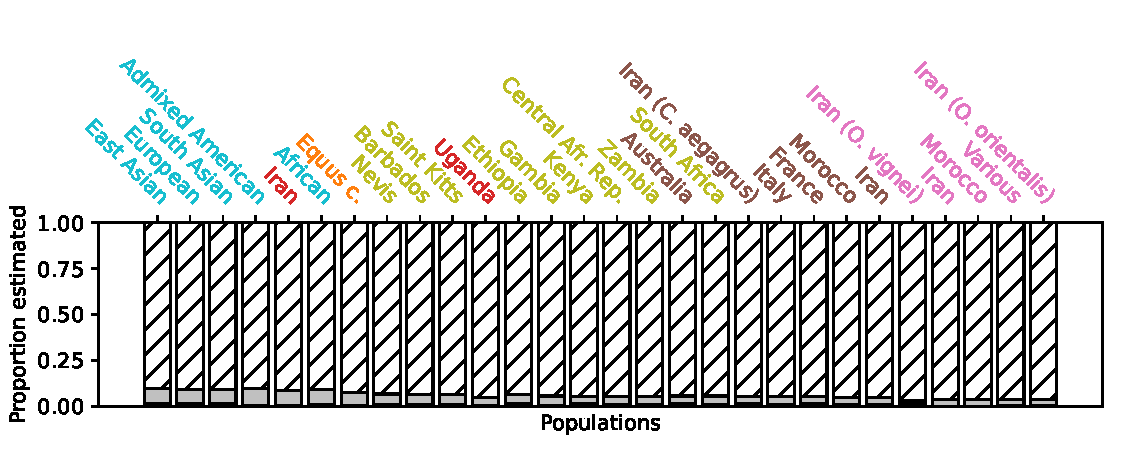
\includegraphics[width=\linewidth, page=1]{artworks/Theta.neg.stacked.pdf}
    \end{minipage}
    \begin{minipage}{0.09\linewidth}
        
\includegraphics[width=\linewidth, page=1]{artworks/legend.polycat}
    \end{minipage}

    \captionof{figure}{Estimation of selection at the population scale for $\SphyNeu$ mutations}
    \begin{minipage}{0.9\linewidth}
        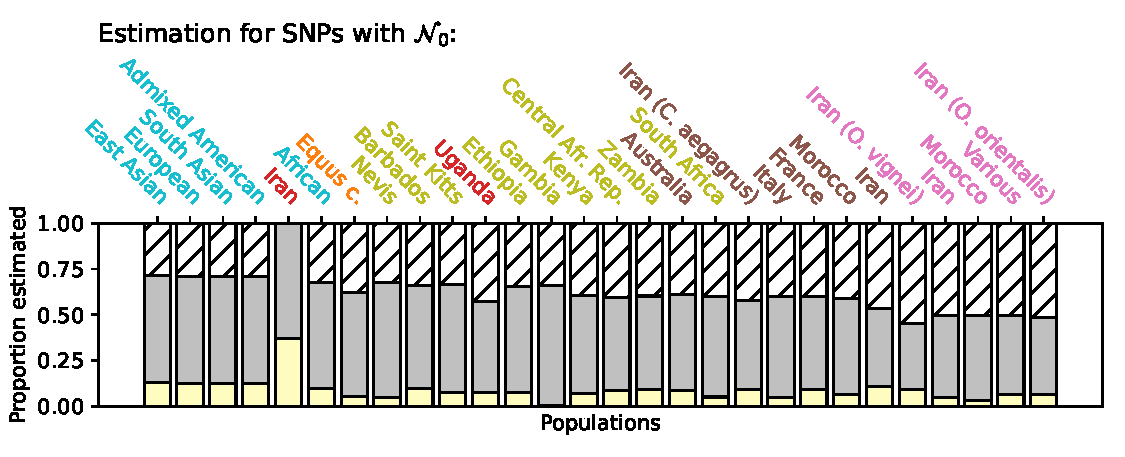
\includegraphics[width=\linewidth, page=1]{artworks/Theta.weak.stacked.pdf}
    \end{minipage}
    \begin{minipage}{0.09\linewidth}
        
\includegraphics[width=\linewidth, page=1]{artworks/legend.polycat}
    \end{minipage}

    \newpage
    \captionof{figure}{Estimation of selection at the population scale for $\SphyBen$ mutations}
    \begin{minipage}{0.9\linewidth}
        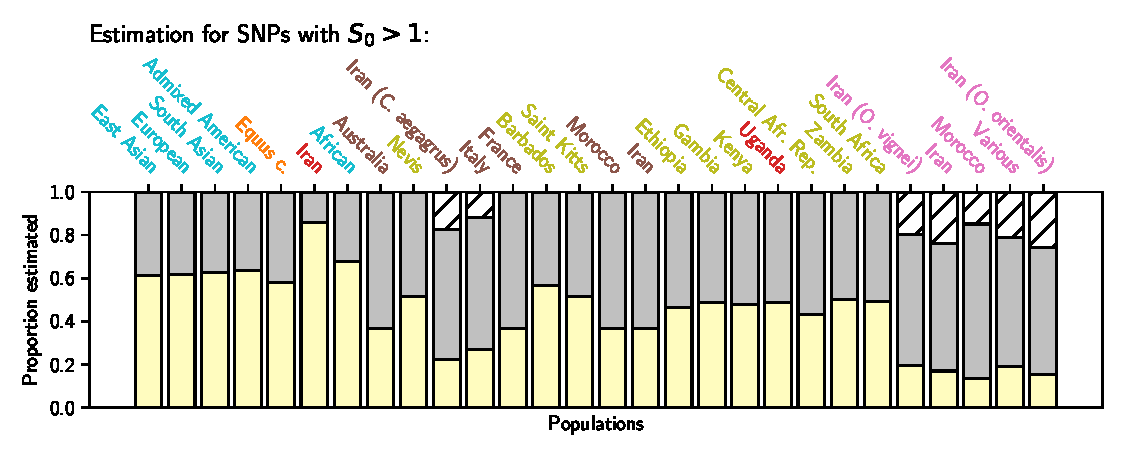
\includegraphics[width=\linewidth, page=1]{artworks/Theta.pos.stacked.pdf}
    \end{minipage}
    \begin{minipage}{0.09\linewidth}
        
\includegraphics[width=\linewidth, page=1]{artworks/legend.polycat}
    \end{minipage}

    \subsection{Correlation with diversity}
    For each population, the proportion of deleterious ($\ProbaPopDel$), nearly-neutral ($\ProbaPopNeu$) and of beneficial ($\ProbaPopBen$) mutations estimated at the population-genetic scale is shown as function of Watterson's's diversity ($\thetaSyn$).

    \subsubsection{Proportion of deleterious mutations ($\SpopDel$)}\label{subsec:proportion-deleterious-mutations}
    \captionof{figure}{Proportion of deleterious mutations ($\SpopDel$)}
    \begin{minipage}{0.49\linewidth}
        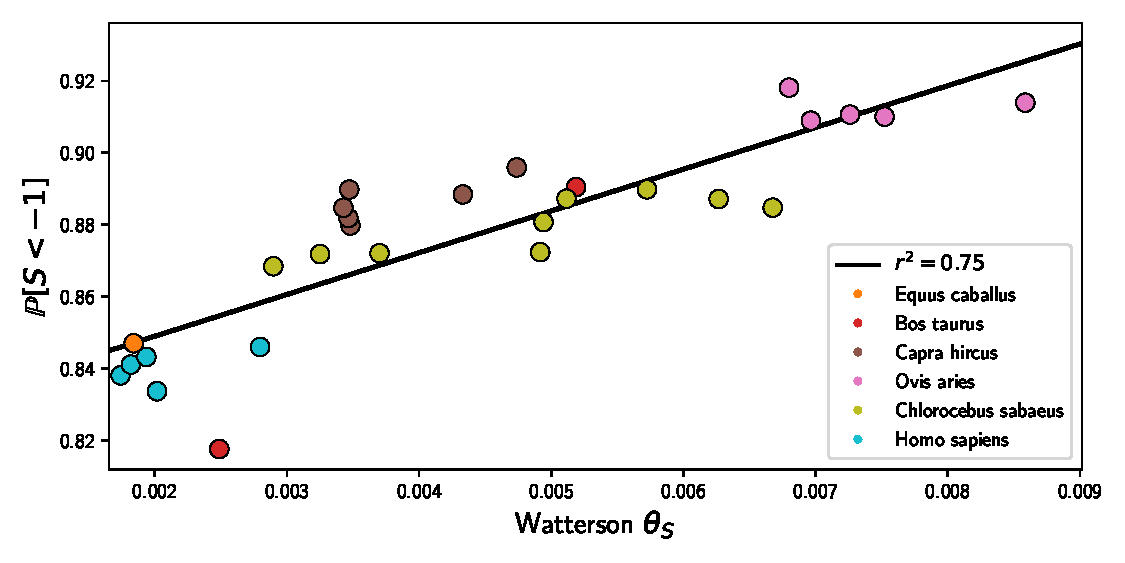
\includegraphics[width=\linewidth, page=1]{artworks/results.watterson.all_P-Sneg.scatter.pdf}
    \end{minipage}
    \begin{minipage}{0.49\linewidth}
        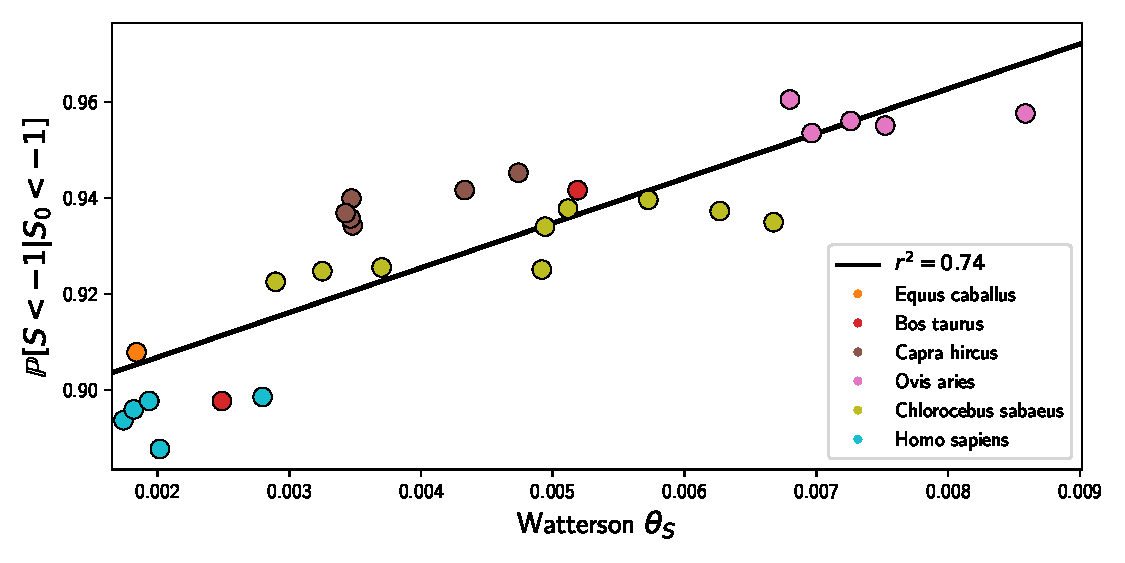
\includegraphics[width=\linewidth, page=1]{artworks/results.watterson.neg_P-Sneg.scatter.pdf}
    \end{minipage}
    \begin{itemize}
        \item Watterson's $\thetaSyn$ is the observed genetic diversity calculated for synonymous changes.
        \item $\proba [ \SpopDel ]$ (computed as eq.~\ref{eq:total_proba} but for $\SpopDel$)  is the probability for a mutation to be deleterious.
        These mutations have a selection coefficient at the population-scale lower than -1.
        \item $\proba [ \SpopDel \given \SphyDel ]$ computed as eq.~\ref{eq:polyProbaAdv} but for $\SpopDel$ and $\SphyDel$) is the probability for a mutation to be deleterious at the population scale, given it is predicted to be a deleterious at the phylogenetic scale.
    \end{itemize}

    We can see that higher synonymous diversity ($\thetaSyn$) is typically accompanied by a higher proportion of effectively deleterious mutations at the population scale ($\proba [ \SpopDel ]$).
    This trend is also confirmed when we restricted the analysis to class of mutations that are supposedly deleterious at the phylogenetic scale ($\SphyDel$).
    This result is qualitatively in accordance with the nearly-neutral theory of evolution which argues that very slightly deleterious mutations are more efficiently purified in large populations.

    \subsubsection{Proportion of nearly-neutral mutations ($\SpopNeu$)}\label{subsec:proportion-nearly-neutral-mutations}
    \captionof{figure}{Proportion of nearly-neutral mutations ($\SpopNeu$)}
    \begin{minipage}{0.49\linewidth}
        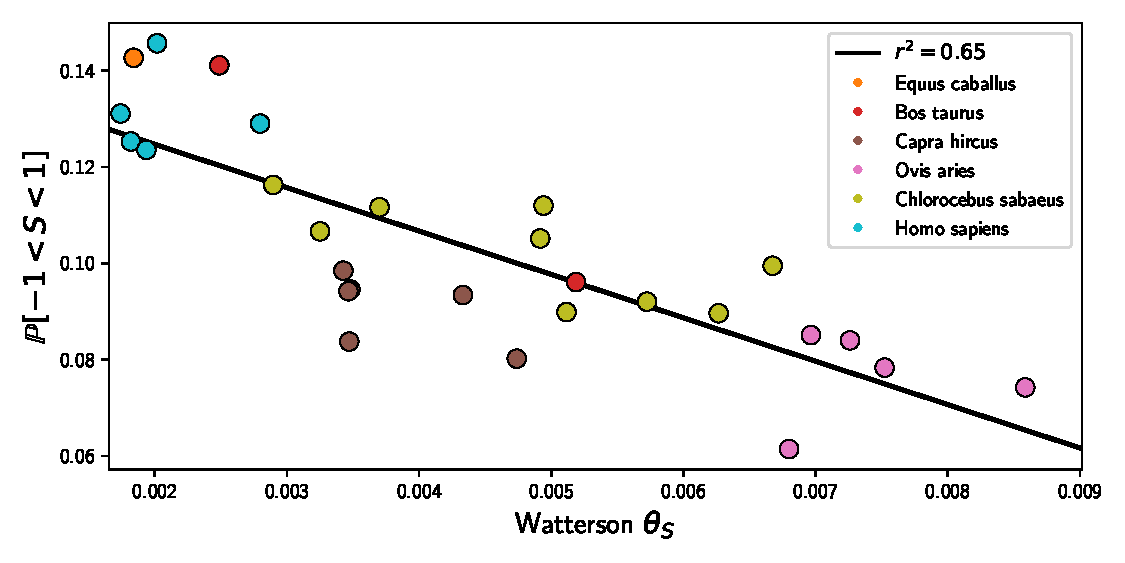
\includegraphics[width=\linewidth, page=1]{artworks/results.watterson.all_P-Sweak.scatter.pdf}
    \end{minipage}
    \begin{minipage}{0.49\linewidth}
        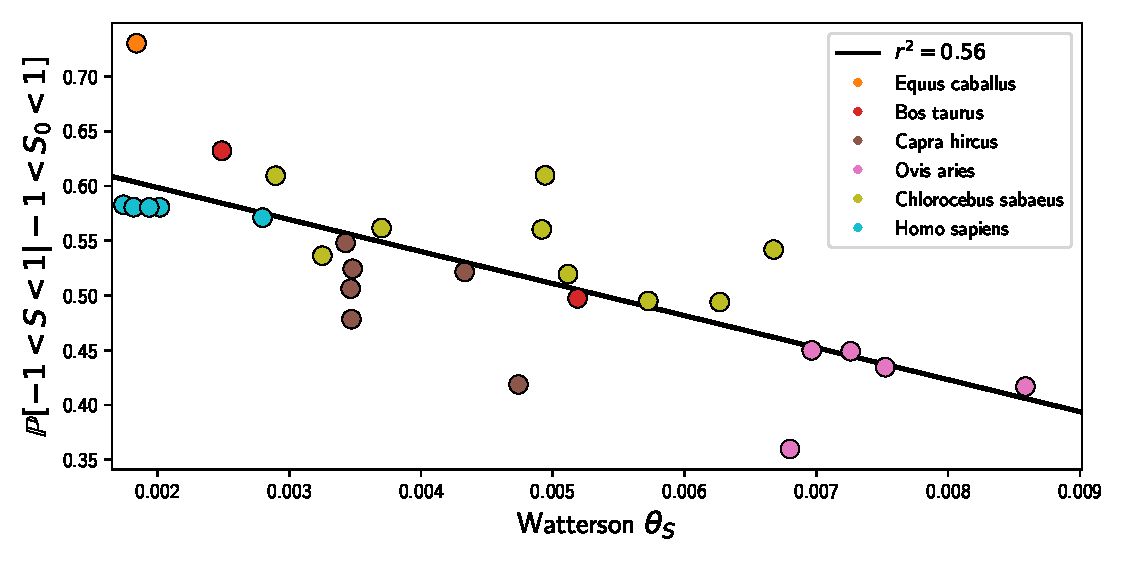
\includegraphics[width=\linewidth, page=1]{artworks/results.watterson.weak_P-Sweak.scatter.pdf}
    \end{minipage}
    \begin{itemize}
        \item Watterson's $\thetaSyn$ is the observed genetic diversity calculated for synonymous changes.
        \item $\proba [ \SpopNeu ]$ (computed as eq.~\ref{eq:total_proba} but for $\SpopNeu$) is the probability for a mutation to be nearly-neutral.
        These mutations have a selection coefficient at the population-scale between -1 and 1.
        \item $\proba [ \SpopNeu \given \SphyNeu ]$ (computed as eq.~\ref{eq:polyProbaAdv} but for $\SpopNeu$ and $\SphyNeu$) is the probability for a mutation to be nearly-neutral at the population scale, given it is predicted to be a nearly-neutral at the phylogenetic scale.
    \end{itemize}

    We confirmed that higher synonymous diversity ($\thetaSyn$) is typically accompanied by a smaller proportion of neutral mutations at the population scale ($\proba [ \SpopNeu ]$ in the range 0.06-0.18).
    This result is more pronounced ($\proba [ \SpopNeu \given \SphyNeu ]$ in the range 0.36-0.73) when we restricted the analysis to class of mutations that are supposedly nearly-neutral at the phylogenetic scale ($\SphyNeu$).
    This result suggests that populations with higher diversity (e.g.~\textit{Bos} or \textit{Ovis}) are more likely to discriminate whether mutations are beneficial or deleterious.
    Alternatively stated, mutations in populations with low diversity (e.g.~\textit{Homo}) are effectively nearly-neutral and behave as would a neutral mutation.
    This result is qualitatively in accordance with the nearly-neutral theory of evolution which argues that mutations are less efficiently selected for in small populations.

    \subsubsection{Proportion of beneficial mutations ($\SpopBen$)}\label{subsec:proportion-beneficial-mutations}
    \captionof{figure}{Proportion of beneficial mutations ($\SpopBen$)}
    \begin{minipage}{0.49\linewidth}
        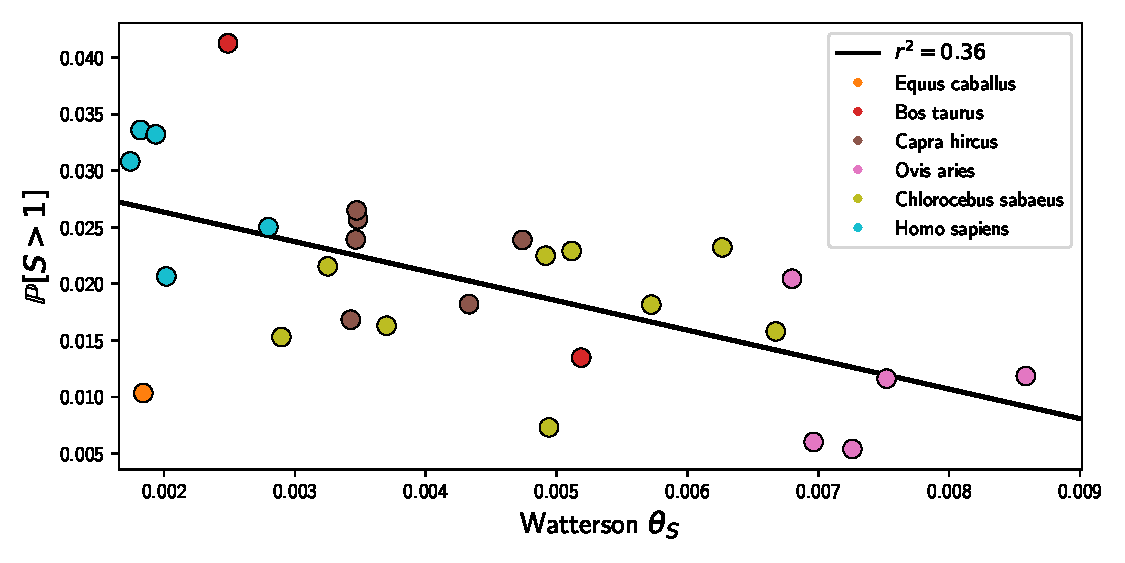
\includegraphics[width=\linewidth, page=1]{artworks/results.watterson.all_P-Spos.scatter.pdf}
    \end{minipage}
    \begin{minipage}{0.49\linewidth}
        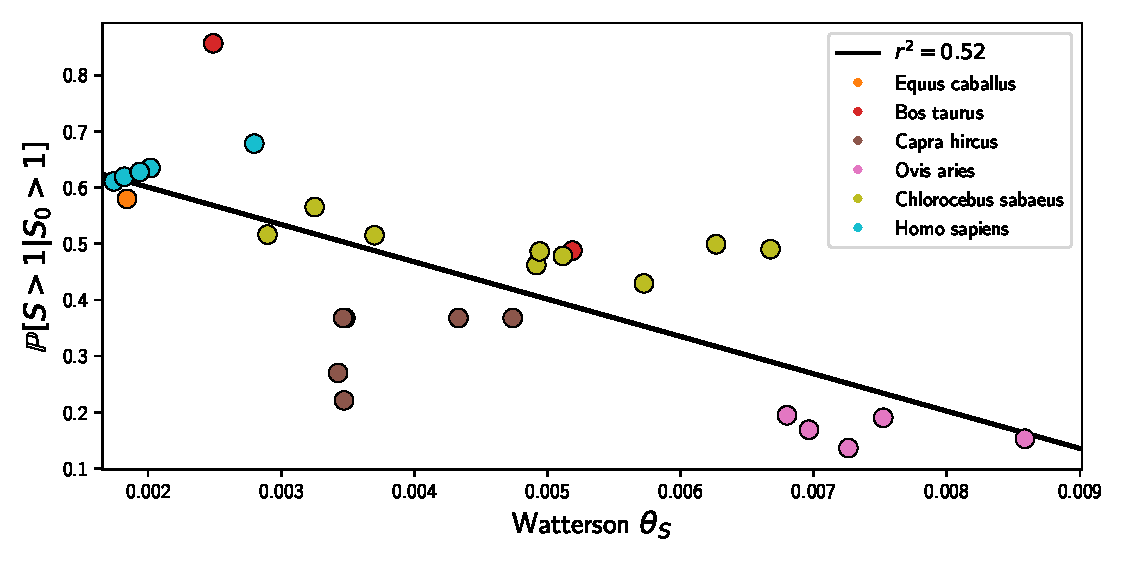
\includegraphics[width=\linewidth, page=1]{artworks/results.watterson.pos_P-Spos.scatter.pdf}
    \end{minipage}
    \begin{itemize}
        \item Watterson's $\thetaSyn$ is the observed genetic diversity calculated for synonymous changes.
        \item $\proba [ \SpopBen ]$ (eq.~\ref{eq:total_proba}) is the probability for a mutation to be beneficial.
        These mutations have a selection coefficient at the population-scale larger than 1.
        \item $\proba [ \SpopBen \given \SphyBen]$ (eq.~\ref{eq:polyProbaAdv}) is the probability for a mutation to be beneficial at the population scale, given it is predicted to be a beneficial back-mutation at the phylogenetic scale (the \textit{precision}).
    \end{itemize}
    Higher synonymous diversity ($\thetaSyn$) is accompanied by a smaller proportion of beneficial mutations at the population scale ($\proba [ \SpopBen ]$).
    This trend is also confirmed when we restricted the analysis to class of mutations that are supposedly beneficial back-mutations at the phylogenetic scale ($\SphyBen$).
    This result is much more difficult to interpret.
    The fraction of beneficial back mutations is supposed to depend on long term demographic history, which is not directly accessible.
    If the long term effective population size is relatively similar to the short term one, we expect little opportunity for beneficial back-mutations.
    And thus, counter-intuitively we expect a diminution of positively selected mutations.
    However, we can see that the proportion of beneficial back-mutations among advantageous one does not decrease with synonymous diversity.
    This means that somehow adaptive mutations also decrease with synonymous diversity for a reason we fail to explain.

    \newpage

    \section{Clinically related terms for mutations}
    \subsection{Terms associated with deleterious mutations $\SphyDel$}
    \begin{center}
        \captionof{table}{Terms associated with deleterious mutations $\SphyDel$}
        \begin{tabular}{|l|r|r|r|r|r|}
            \toprule
            SNP clinical ontology & $n_{\mathrm{Observed}}$ & $n_{\mathrm{Expected}}$ & Odds ratio & $p_{\mathrm{v}}$ & $p_{\mathrm{v-adjusted}}$ \\
            \midrule
            Benign                & 2969                    & $4043.0$                & $ 0.734$   & $ 1.000$             & $ 1.000~~$                    \\
            Likely benign         & 2994                    & $3399.8$                & $ 0.881$   & $ 0.999$             & $ 1.000~~$                    \\
            Risk factor           & 102                     & $ 118.2$                & $ 0.863$   & $ 0.798$             & $ 1.000~~$                    \\
            Likely pathogenic     & 221                     & $  68.5$                  & $ 3.226$   & $1.7\times 10^{-8}$  & $\bm{6.7\times 10^{-8}{^*}}$  \\
            Pathogenic            & 560                     & $ 193.6$                & $ 2.893$   & $4.2\times 10^{-17}$ & $\bm{2.1\times 10^{-16}{^*}}$ \\
            \bottomrule
        \end{tabular}
    \end{center}
    In humans, non-synonymous SNPs in the test group ($\SphyDel$) are contrasted to SNPs in the control group ($\SphyNeu$).
    For each clinical term, a 2x2 contingency tables is built by counting the number of SNPs based on their selection coefficient and their clinical terms (whether they have this specific term or not).
    Fisher's exact tests are then performed for these 2x2 contingency tables.
    $^*$ for $p_{\mathrm{v}}^{\mathrm{adj}}$ corrected for multiple comparison (Holm–Bonferroni correction) lower than the risk $\alpha=0.05$.
    SNPs predicted with $\SphyDel$ are statistically associated to clinical terms such as \textit{Likely Pathogenic} and \textit{Pathogenic}.

    \subsection{Terms associated with beneficial back-mutations $\SphyBen$}
    \begin{center}
        \captionof{table}{Terms associated with beneficial back-mutations $\SphyBen$}
        \begin{tabular}{|l|r|r|r|r|r|}
            \toprule
            SNP clinical ontology & $n_{\mathrm{Observed}}$ & $n_{\mathrm{Expected}}$ & Odds ratio & $p_{\mathrm{v}}$ & $p_{\mathrm{v-adjusted}}$ \\
            \midrule
            Benign                & 319                     & $ 261.7$                & $ 1.219$   & $ 0.002$         & $\bm{ 0.009{^*}}$         \\
            Likely benign         & 263                     & $ 222.7$                & $ 1.181$   & $ 0.012$         & $\bm{ 0.049{^*}}$         \\
            Risk factor           & 5                       & $ 7.847$                & $ 0.637$   & $ 0.879$         & $ 0.879~~$                \\
            Likely pathogenic     & 7                       & $ 4.552$                & $ 1.538$   & $ 0.227$         & $ 0.682~~$                \\
            Pathogenic            & 16                      & $  12.9$                  & $ 1.241$   & $ 0.268$         & $ 0.682~~$                \\
            \bottomrule
        \end{tabular}
    \end{center}
    In humans, non-synonymous SNPs in the test group ($\SphyBen$) are contrasted to SNPs in the control group ($\SphyNeu$).
    For each clinical term, a 2x2 contingency tables is built by counting the number of SNPs based on their selection coefficient and their clinical terms (whether they have this specific term or not).
    Fisher's exact tests are then performed for these 2x2 contingency tables.
    $^*$ for $p_{\mathrm{v}}^{\mathrm{adj}}$ corrected for multiple comparison (Holm–Bonferroni correction) lower than the risk $\alpha=0.05$.
    Beneficial back-mutations are associated with clinical terms such as \textit{Benign} and \textit{Likely Benign}.
    \newpage

    \section{Including divergence data for the estimation of $\Spop$}

    \subsection{Including divergence in polyDFE}
    Divergence data (number of substitutions per site) can also be included into polyDFE to estimate the DFE.
    For the class of a given class of selection coefficient ($\Sphyclass \in \{\SphyDel, \SphyNeu, \SphyBen \}$), the number of substitutions has already been computed and is given by $D\left( \Sphyclass \right)$ (see eq.~\ref{eq:dnds}), and the number of sites is given by $L \left( \Sphyclass \right)$ (see eq.~\ref{eq:mutation-opp}).
    Otherwise, the procedure is the same as described section \textit{Scaled selection coefficients ($\Spop$) in a population-based method}.

    \subsection{Probabilities of beneficial back-mutations}
    \begin{center}
        \captionof{table}{Probability of beneficial back-mutations among all beneficial ones.}
        \scriptsize
        \begin{longtable*}{|l|l|r|r|r|r|r|r|}
            \toprule
            Population & Species & Watterson's $\thetaSyn$ & $\proba[\SphyBen]$ & $\proba [ \SpopBen ]$ & $\frac{\proba[\SphyBen]}{\proba[ \SpopBen ]}$ & $\proba [ \SpopBen \given \SphyBen]$ & $\proba[\SphyBen\given \SpopBen ]$ \\
            \midrule
            \endhead
            \midrule
            \multicolumn{8}{r}{{Continued on next page}} \\
            \midrule
            \endfoot

            \bottomrule
            \endlastfoot
            \rowcolor{LIGHTGREY} Equus c. &      Equus caballus &               $ 0.002$ &              $ 0.014$ &              $ 0.061$ &                                          $ 0.235$ &                         $ 0.519$ &                      $ 0.122$ \\
            Iran &          Bos taurus &               $ 0.002$ &              $ 0.013$ &              $ 0.007$ &                                          $ 1.908$ &                         $ 0.368$ &                      $ 0.702$ \\
            Uganda &          Bos taurus &               $ 0.005$ &              $ 0.013$ &              $ 0.008$ &                                          $ 1.667$ &                         $ 0.255$ &                      $ 0.425$ \\
            \rowcolor{LIGHTGREY} Australia &        Capra hircus &               $ 0.003$ &              $ 0.014$ &              $ 0.007$ &                                          $ 2.099$ &                         $ 0.147$ &                      $ 0.308$ \\
            \rowcolor{LIGHTGREY} France &        Capra hircus &               $ 0.004$ &              $ 0.014$ &              $ 0.007$ &                                          $ 2.043$ &                         $ 0.149$ &                      $ 0.304$ \\
            \rowcolor{LIGHTGREY} Iran (C. aegagrus) &        Capra hircus &               $ 0.004$ &              $ 0.014$ &              $ 0.013$ &                                          $ 1.069$ &                         $ 0.147$ &                      $ 0.157$ \\
            \rowcolor{LIGHTGREY} Iran &        Capra hircus &               $ 0.004$ &              $ 0.014$ &              $ 0.008$ &                                          $ 1.699$ &                         $ 0.152$ &                      $ 0.258$ \\
            \rowcolor{LIGHTGREY} Italy &        Capra hircus &               $ 0.004$ &              $ 0.014$ &              $ 0.006$ &                                          $ 2.160$ &                         $ 0.147$ &                      $ 0.316$ \\
            \rowcolor{LIGHTGREY} Morocco &        Capra hircus &               $ 0.004$ &              $ 0.014$ &              $ 0.006$ &                                          $ 2.141$ &                         $ 0.186$ &                      $ 0.398$ \\
            Iran &          Ovis aries &               $ 0.007$ &              $ 0.014$ &              $ 0.012$ &                                          $ 1.210$ &                         $ 0.158$ &                      $ 0.191$ \\
            Iran (O. orientalis) &          Ovis aries &               $ 0.009$ &              $ 0.014$ &              $ 0.012$ &                                          $ 1.144$ &                         $ 0.157$ &                      $ 0.180$ \\
            Iran (O. vignei) &          Ovis aries &               $ 0.007$ &              $ 0.014$ &              $ 0.022$ &                                          $ 0.631$ &                         $ 0.186$ &                      $ 0.118$ \\
            Various &          Ovis aries &               $ 0.008$ &              $ 0.014$ &              $ 0.012$ &                                          $ 1.211$ &                         $ 0.156$ &                      $ 0.188$ \\
            Morocco &          Ovis aries &               $ 0.008$ &              $ 0.014$ &              $ 0.009$ &                                          $ 1.536$ &                         $ 0.190$ &                      $ 0.292$ \\
            \rowcolor{LIGHTGREY} Barbados & Chlorocebus sabaeus &               $ 0.004$ &              $ 0.012$ &              $ 0.005$ &                                          $ 2.230$ &                         $ 0.282$ &                      $ 0.630$ \\
            \rowcolor{LIGHTGREY} Central Afr. Rep. & Chlorocebus sabaeus &               $ 0.006$ &              $ 0.012$ &              $ 0.014$ &                                          $ 0.849$ &                         $ 0.310$ &                      $ 0.263$ \\
            \rowcolor{LIGHTGREY} Ethiopia & Chlorocebus sabaeus &               $ 0.005$ &              $ 0.012$ &              $ 0.008$ &                                          $ 1.530$ &                         $ 0.298$ &                      $ 0.456$ \\
            \rowcolor{LIGHTGREY} Gambia & Chlorocebus sabaeus &               $ 0.005$ &              $ 0.012$ &              $ 0.008$ &                                          $ 1.384$ &                         $ 0.305$ &                      $ 0.422$ \\
            \rowcolor{LIGHTGREY} Kenya & Chlorocebus sabaeus &               $ 0.005$ &              $ 0.012$ &              $ 0.014$ &                                          $ 0.854$ &                         $ 0.296$ &                      $ 0.253$ \\
            \rowcolor{LIGHTGREY} Nevis & Chlorocebus sabaeus &               $ 0.003$ &              $ 0.012$ &              $ 0.005$ &                                          $ 2.438$ &                         $ 0.285$ &                      $ 0.696$ \\
            \rowcolor{LIGHTGREY} South Africa  & Chlorocebus sabaeus &               $ 0.006$ &              $ 0.012$ &              $ 0.011$ &                                          $ 1.047$ &                         $ 0.323$ &                      $ 0.338$ \\
            \rowcolor{LIGHTGREY} Saint Kitts & Chlorocebus sabaeus &               $ 0.004$ &              $ 0.012$ &              $ 0.006$ &                                          $ 2.070$ &                         $ 0.292$ &                      $ 0.604$ \\
            \rowcolor{LIGHTGREY} Zambia & Chlorocebus sabaeus &               $ 0.006$ &              $ 0.012$ &              $ 0.014$ &                                          $ 0.816$ &                         $ 0.309$ &                      $ 0.252$ \\
            African &        Homo sapiens &               $ 0.002$ &              $ 0.012$ &              $ 0.015$ &                                          $ 0.765$ &                         $ 0.371$ &                      $ 0.284$ \\
            Admixed American &        Homo sapiens &               $ 0.002$ &              $ 0.012$ &              $ 0.009$ &                                          $ 1.259$ &                         $ 0.368$ &                      $ 0.464$ \\
            East Asian &        Homo sapiens &               $ 0.002$ &              $ 0.012$ &              $ 0.012$ &                                          $ 0.973$ &                         $ 0.369$ &                      $ 0.358$ \\
            European &        Homo sapiens &               $ 0.002$ &              $ 0.012$ &              $ 0.009$ &                                          $ 1.356$ &                         $ 0.368$ &                      $ 0.499$ \\
            South Asian &        Homo sapiens &               $ 0.002$ &              $ 0.012$ &              $ 0.010$ &                                          $ 1.147$ &                         $ 0.369$ &                      $ 0.423$ \\
        \end{longtable*}
    \end{center}
    \begin{itemize}
        \item Watterson's $\thetaSyn$ is the observed genetic diversity calculated for synonymous changes.
        \item $\proba [ \SphyBen ]$ (eq.~\ref{eq:proba-dfe-mutsel}) is the probability for a new mutation a beneficial back-mutation.
        These mutations have a selection coefficient predicted at the phylogenetic-scale larger than 1, thus toward a more fit amino-acid.
        \item $\proba [ \SpopBen ]$ (eq.~\ref{eq:total_proba}) is the probability for a mutation to be beneficial.
        These mutations have a selection coefficient at the population-scale larger than 1.
        \item $\proba [ \SpopBen \given \SphyBen]$ (eq.~\ref{eq:polyProbaAdv}) is the probability for a mutation to be beneficial at the population scale, given it is predicted to be a beneficial back-mutation at the phylogenetic scale (the \textit{precision}).
        \item $\proba [ \SphyBen \given \SpopBen]$ (eq.~\ref{eq:bayes}) is the probability for a mutation to a beneficial back-mutations, given it is beneficial (the \textit{recall}).
        This probability is obtained using Bayes' formula.
    \end{itemize}
    \newpage

    \subsection{Precision and recall}
    \captionof{table}{Precision and recall}
    \begin{center}
        \begin{adjustbox}{width=\textwidth}
            \begin{tabular}{||l|l|r||r|r||r|r||r|r||}
                \toprule
                \multicolumn{3}{||c||}{} &
                \multicolumn{2}{c||}{\shortstack{\textbf{Deleterious mutations} \\ $\bm{\SpopDel \coloneqq \Spop<-1}$ \\ $\bm{\SphyDel \coloneqq \Sphy<-1}$}} &
                \multicolumn{2}{c||}{\shortstack{\textbf{Nearly-neutral mutations} \\ $\bm{\SpopNeu \coloneqq -1<\Spop<1}$ \\ $\bm{\SphyNeu \coloneqq -1<\Sphy<1}$}} &
                \multicolumn{2}{c||}{\shortstack{\textbf{Beneficial mutations} \\ $\bm{\SpopBen \coloneqq \Spop>1}$ \\ $\bm{\SphyBen \coloneqq \Sphy>1}$}}
                \\ \hline
                \textbf{Population} &
                \textbf{Species} &
                $\bm{\thetaSyn}$ &
                \makecell{\textbf{Precision} \\ $\bm{\proba [\SpopDel \given \SphyDel]}$} &
                \makecell{\textbf{Recall} \\ $\bm{\proba [\SphyDel \given \SpopDel]}$}           &
                \makecell{\textbf{Precision}      \\ $\bm{\proba [\SpopNeu \given \SphyNeu]}$}                                    &
                \makecell{\textbf{Recall}          \\ $\bm{\proba [\SphyNeu \given \SpopNeu]}$}                                  &
                \makecell{\textbf{Precision}          \\ $\bm{\proba [\SpopBen \given \SphyBen]}$}          &
                \makecell{\textbf{Recall}        \\ $\bm{\proba [\SphyBen \given \SpopBen]}$}
                \\   \midrule
                \rowcolor{LIGHTGREY} Equus c. & Equus caballus        & $ 0.002$ & $ 0.918$ & $ 0.957$ & $ 0.186$ & $ 0.213$ & $ 0.519$ & $ 0.122$ \\
                Iran               & Bos taurus        & $ 0.002$ & $ 0.924$ & $ 0.965$ & $ 0.565$ & $ 0.356$ & $ 0.368$ & $ 0.702$ \\
                Uganda              & Bos taurus        & $ 0.005$ & $ 0.943$ & $ 0.961$ & $ 0.516$ & $ 0.396$ & $ 0.255$ & $ 0.425$ \\
                \rowcolor{LIGHTGREY} Australia            & Capra hircus        & $ 0.003$ & $ 0.941$ & $ 0.964$ & $ 0.592$ & $ 0.434$ & $ 0.147$ & $ 0.308$ \\
                \rowcolor{LIGHTGREY} France                                    & Capra hircus          & $ 0.004$ & $ 0.940$ & $ 0.963$ & $ 0.571$ & $ 0.418$ & $ 0.149$ & $ 0.304$ \\
                \rowcolor{LIGHTGREY} Iran (C. aegagrus)                    & Capra hircus          & $ 0.004$ & $ 0.948$ & $ 0.960$ & $ 0.515$ & $ 0.446$ & $ 0.147$ & $ 0.157$ \\
                \rowcolor{LIGHTGREY} Iran                        & Capra hircus          & $ 0.004$ & $ 0.942$ & $ 0.961$ & $ 0.534$ & $ 0.410$ & $ 0.152$ & $ 0.258$ \\
                \rowcolor{LIGHTGREY} Italy                                 & Capra hircus          & $ 0.004$ & $ 0.940$ & $ 0.963$ & $ 0.579$ & $ 0.421$ & $ 0.147$ & $ 0.316$ \\
                \rowcolor{LIGHTGREY} Morocco                                 & Capra hircus          & $ 0.004$ & $ 0.939$ & $ 0.960$ & $ 0.549$ & $ 0.404$ & $ 0.186$ & $ 0.398$ \\
                Iran           & Ovis aries & $ 0.007$ & $ 0.957$ & $ 0.954$ & $ 0.412$ & $ 0.416$ & $ 0.158$ & $ 0.191$ \\
                Iran (O. orientalis)  & Ovis aries & $ 0.009$ & $ 0.961$ & $ 0.955$ & $ 0.413$ & $ 0.437$ & $ 0.157$ & $ 0.180$ \\
                Iran (O. vignei)           & Ovis aries & $ 0.007$ & $ 0.968$ & $ 0.951$ & $ 0.356$ & $ 0.516$ & $ 0.186$ & $ 0.118$ \\
                Various             & Ovis aries & $ 0.008$ & $ 0.958$ & $ 0.955$ & $ 0.428$ & $ 0.431$ & $ 0.156$ & $ 0.188$ \\
                Morocco              & Ovis aries & $ 0.008$ & $ 0.960$ & $ 0.953$ & $ 0.447$ & $ 0.460$ & $ 0.190$ & $ 0.292$ \\
                \rowcolor{LIGHTGREY} Barbados              & Chlorocebus sabaeus & $ 0.004$ & $ 0.931$ & $ 0.969$ & $ 0.628$ & $ 0.402$ & $ 0.282$ & $ 0.630$ \\
                \rowcolor{LIGHTGREY} Central Afr. Rep.       & Chlorocebus sabaeus & $ 0.006$ & $ 0.941$ & $ 0.964$ & $ 0.514$ & $ 0.408$ & $ 0.310$ & $ 0.263$ \\
                \rowcolor{LIGHTGREY} Ethiopia        & Chlorocebus sabaeus & $ 0.005$ & $ 0.933$ & $ 0.967$ & $ 0.586$ & $ 0.393$ & $ 0.298$ & $ 0.456$ \\
                \rowcolor{LIGHTGREY} Gambia             & Chlorocebus sabaeus & $ 0.005$ & $ 0.937$ & $ 0.967$ & $ 0.590$ & $ 0.414$ & $ 0.305$ & $ 0.422$ \\
                \rowcolor{LIGHTGREY} Kenya                                 & Chlorocebus sabaeus        & $ 0.005$ & $ 0.942$ & $ 0.965$ & $ 0.526$ & $ 0.418$ & $ 0.296$ & $ 0.253$ \\
                \rowcolor{LIGHTGREY} Nevis                        & Chlorocebus sabaeus        & $ 0.003$ & $ 0.930$ & $ 0.970$ & $ 0.637$ & $ 0.401$ & $ 0.285$ & $ 0.696$ \\
                \rowcolor{LIGHTGREY} South Africa                              & Chlorocebus sabaeus        & $ 0.006$ & $ 0.937$ & $ 0.964$ & $ 0.530$ & $ 0.393$ & $ 0.323$ & $ 0.338$ \\
                \rowcolor{LIGHTGREY} Saint Kitts                                & Chlorocebus sabaeus        & $ 0.004$ & $ 0.931$ & $ 0.969$ & $ 0.611$ & $ 0.393$ & $ 0.292$ & $ 0.604$ \\
                \rowcolor{LIGHTGREY} Zambia                             & Chlorocebus sabaeus        & $ 0.006$ & $ 0.941$ & $ 0.963$ & $ 0.506$ & $ 0.408$ & $ 0.309$ & $ 0.252$ \\
                African                             & Homo sapiens        & $ 0.002$ & $ 0.896$ & $ 0.968$ & $ 0.550$ & $ 0.297$ & $ 0.371$ & $ 0.284$ \\
                Admixed American                             & Homo sapiens        & $ 0.002$ & $ 0.890$ & $ 0.979$ & $ 0.710$ & $ 0.333$ & $ 0.368$ & $ 0.464$ \\
                East Asian                             & Homo sapiens        & $ 0.002$ & $ 0.890$ & $ 0.971$ & $ 0.578$ & $ 0.289$ & $ 0.369$ & $ 0.358$ \\
                European                             & Homo sapiens        & $ 0.002$ & $ 0.891$ & $ 0.980$ & $ 0.739$ & $ 0.345$ & $ 0.368$ & $ 0.499$ \\
                South Asian                             & Homo sapiens        & $ 0.002$ & $ 0.895$ & $ 0.981$ & $ 0.740$ & $ 0.356$ & $ 0.369$ & $ 0.423$ \\
                \bottomrule
            \end{tabular}
        \end{adjustbox}
    \end{center}
    \begin{itemize}
        \item Watterson's $\thetaSyn$ is the observed genetic diversity calculated for synonymous changes.
        \item \textit{Precision} is the estimation of the selection coefficient at population scale ($\Spop$) given that $\Sphy$ is known.
        \item  \textit{Recall} is the estimation of $\Sphy$ given selection coefficient at the population scale ($\Spop$) is known.
        \item \textit{Recall} for beneficial mutations ($\proba [\SphyBen \given \SpopBen]$) is thus the proportion of beneficial back-mutations among all beneficial mutations.
    \end{itemize}

    Altogether, comparing this table to tables 1 and S3, we acknowledge that the exact proportion of beneficial back-mutations among all beneficial ones is different whether we included or not substitutions in the terminal lineage for the estimation of $\Spop$.
    However, we can still see that beneficial back-mutations are positively selected compared to neutral and deleterious ones, and this result is not sensitive to inclusion of substitutions in the terminal lineage.

    \newpage
    \section{Discrete distribution of $\Spop$ at the population scale}

    \subsection{polyDFE model D (discrete distribution)}
    With polyDFE model D, the DFE of non-synonymous mutations is given as a discrete DFE of $K$ categories (instead of a continuous distribution in model C), where the selection coefficients of each category $i$ ($1 \leq i \leq K$) are fixed parameters $\Spop_i$, and each value $\Spop_i$ has a probability $p_i$ (estimated), with $\sum_{i=1}^{K} p_i =1$.
    We used $K=6$ with $\Spop_1 = -500$, $\Spop_2 = -4$, $\Spop_3 =-1$, $\Spop_4 = 0$, $\Spop_5 = 1$, $\Spop_6 = 4$.\\
    For each class of selection $\Sphyclass$, the parameters $p_i$ ($i \in \{ 1 \leq i \leq 6 \}$) were used to compute $\proba [ \SpopDel \given  \Sphyclass] $, $\proba [ \SpopNeu \given \Sphyclass]$, and $\proba [ \SpopBen \given \Sphyclass]$ as:
    \begin{align}
        \proba [ \SpopDel \given  \Sphyclass] &= \proba [ \Spop < -1 \given \Sphyclass ] = p_1 + p_2 \label{eq:polyProbaDel-mD} \\
        \proba [ \SpopNeu \given \Sphyclass] &= \proba [ -1 < \Spop < 1 \given \Sphyclass ] = p_3 + p_4 + p_5,  \\
        \proba [ \SpopBen \given \Sphyclass] &= p_6. \label{eq:polyProbaAdv-mD}
    \end{align}

    \subsection{Probabilities of beneficial back-mutations}
    \begin{center}
        \captionof{table}{Probability of beneficial back-mutations among all beneficial ones.}
        \scriptsize
        \begin{longtable*}{|l|l|r|r|r|r|r|r|}
            \toprule
            Population & Species & Watterson's $\thetaSyn$ & $\proba[\SphyBen]$ & $\proba [ \SpopBen ]$ & $\frac{\proba[\SphyBen]}{\proba[ \SpopBen ]}$ & $\proba [ \SpopBen \given \SphyBen]$ & $\proba[\SphyBen\given \SpopBen ]$ \\
            \midrule
            \endhead
            \midrule
            \multicolumn{8}{r}{{Continued on next page}} \\
            \midrule
            \endfoot

            \bottomrule
            \endlastfoot
            \rowcolor{LIGHTGREY} Equus c. &      Equus caballus &               $ 0.002$ &              $ 0.014$ &              $ 0.006$ &                                          $ 2.230$ &                         $ 0.141$ &                      $ 0.316$ \\
            Iran &          Bos taurus &               $ 0.002$ &              $ 0.013$ &              $ 0.006$ &                                          $ 2.200$ &                         $ 0.136$ &                      $ 0.298$ \\
            Uganda &          Bos taurus &               $ 0.005$ &              $ 0.013$ &              $ 0.011$ &                                          $ 1.177$ &                         $ 0.138$ &                      $ 0.162$ \\
            \rowcolor{LIGHTGREY} Australia &        Capra hircus &               $ 0.003$ &              $ 0.014$ &              $ 0.002$ &                                          $ 6.467$ &                         $ 0.135$ &                      $ 0.871$ \\
            \rowcolor{LIGHTGREY} France &        Capra hircus &               $ 0.004$ &              $ 0.014$ &              $ 0.002$ &                                          $ 6.407$ &                         $ 0.132$ &                      $ 0.845$ \\
            \rowcolor{LIGHTGREY} Iran (C. aegagrus) &        Capra hircus &               $ 0.004$ &              $ 0.014$ &              $ 0.002$ &                                          $ 5.993$ &                         $ 0.129$ &                      $ 0.772$ \\
            \rowcolor{LIGHTGREY} Iran &        Capra hircus &               $ 0.004$ &              $ 0.014$ &              $ 0.004$ &                                          $ 3.656$ &                         $ 0.138$ &                      $ 0.506$ \\
            \rowcolor{LIGHTGREY} Italy &        Capra hircus &               $ 0.004$ &              $ 0.014$ &              $ 0.002$ &                                          $ 6.216$ &                         $ 0.127$ &                      $ 0.787$ \\
            \rowcolor{LIGHTGREY} Morocco &        Capra hircus &               $ 0.004$ &              $ 0.014$ &              $ 0.002$ &                                          $ 6.019$ &                         $ 0.141$ &                      $ 0.848$ \\
            Iran &          Ovis aries &               $ 0.007$ &              $ 0.014$ &              $ 0.024$ &                                          $ 0.588$ &                         $ 0.148$ &                      $ 0.087$ \\
            Iran (O. orientalis) &          Ovis aries &               $ 0.009$ &              $ 0.014$ &              $ 0.024$ &                                          $ 0.569$ &                         $ 0.143$ &                      $ 0.081$ \\
            Iran (O. vignei) &          Ovis aries &               $ 0.007$ &              $ 0.014$ &              $ 0.024$ &                                          $ 0.587$ &                         $ 0.127$ &                      $ 0.075$ \\
            Various &          Ovis aries &               $ 0.008$ &              $ 0.014$ &              $ 0.024$ &                                          $ 0.588$ &                         $ 0.146$ &                      $ 0.086$ \\
            Morocco &          Ovis aries &               $ 0.008$ &              $ 0.014$ &              $ 0.025$ &                                          $ 0.564$ &                         $ 0.145$ &                      $ 0.082$ \\
            \rowcolor{LIGHTGREY} Barbados & Chlorocebus sabaeus &               $ 0.004$ &              $ 0.012$ &              $ 0.002$ &                                          $ 5.689$ &                         $ 0.170$ &                      $ 0.968$ \\
            \rowcolor{LIGHTGREY} Central Afr. Rep. & Chlorocebus sabaeus &               $ 0.006$ &              $ 0.012$ &              $ 0.005$ &                                          $ 2.142$ &                         $ 0.156$ &                      $ 0.334$ \\
            \rowcolor{LIGHTGREY} Ethiopia & Chlorocebus sabaeus &               $ 0.005$ &              $ 0.012$ &              $ 0.002$ &                                          $ 5.910$ &                         $ 0.160$ &                      $ 0.945$ \\
            \rowcolor{LIGHTGREY} Gambia & Chlorocebus sabaeus &               $ 0.005$ &              $ 0.012$ &              $ 0.006$ &                                          $ 1.850$ &                         $ 0.157$ &                      $ 0.290$ \\
            \rowcolor{LIGHTGREY} Kenya & Chlorocebus sabaeus &               $ 0.005$ &              $ 0.012$ &              $ 0.004$ &                                          $ 2.802$ &                         $ 0.163$ &                      $ 0.456$ \\
            \rowcolor{LIGHTGREY} Nevis & Chlorocebus sabaeus &               $ 0.003$ &              $ 0.012$ &              $ 0.002$ &                                          $ 5.396$ &                         $ 0.169$ &                      $ 0.910$ \\
            \rowcolor{LIGHTGREY} South Africa & Chlorocebus sabaeus &               $ 0.006$ &              $ 0.012$ &              $ 0.005$ &                                          $ 2.154$ &                         $ 0.153$ &                      $ 0.329$ \\
            \rowcolor{LIGHTGREY} Saint Kitts & Chlorocebus sabaeus &               $ 0.004$ &              $ 0.012$ &              $ 0.002$ &                                          $ 5.094$ &                         $ 0.164$ &                      $ 0.834$ \\
            \rowcolor{LIGHTGREY} Zambia & Chlorocebus sabaeus &               $ 0.006$ &              $ 0.012$ &              $ 0.006$ &                                          $ 1.952$ &                         $ 0.153$ &                      $ 0.298$ \\
            African &        Homo sapiens &               $ 0.002$ &              $ 0.012$ &              $ 0.014$ &                                          $ 0.869$ &                         $ 0.141$ &                      $ 0.123$ \\
            Admixed American &        Homo sapiens &               $ 0.002$ &              $ 0.012$ &              $ 0.010$ &                                          $ 1.130$ &                         $ 0.161$ &                      $ 0.182$ \\
            East Asian &        Homo sapiens &               $ 0.002$ &              $ 0.012$ &              $ 0.007$ &                                          $ 1.602$ &                         $ 0.162$ &                      $ 0.259$ \\
            European &        Homo sapiens &               $ 0.002$ &              $ 0.012$ &              $ 0.009$ &                                          $ 1.336$ &                         $ 0.163$ &                      $ 0.217$ \\
            South Asian &        Homo sapiens &               $ 0.002$ &              $ 0.012$ &              $ 0.009$ &                                          $ 1.342$ &                         $ 0.163$ &                      $ 0.219$ \\
        \end{longtable*}
    \end{center}
    \begin{itemize}
        \item Watterson's $\thetaSyn$ is the observed genetic diversity calculated for synonymous changes.
        \item $\proba [ \SphyBen ]$ (eq.~\ref{eq:proba-dfe-mutsel}) is the probability for a new mutation a beneficial back-mutation.
        These mutations have a selection coefficient predicted at the phylogenetic-scale larger than 1, thus toward a more fit amino-acid.
        \item $\proba [ \SpopBen ]$ (eq.~\ref{eq:total_proba}) is the probability for a mutation to be beneficial.
        These mutations have a selection coefficient at the population-scale larger than 1.
        \item $\proba [ \SpopBen \given \SphyBen]$ (eq.~\ref{eq:polyProbaAdv}) is the probability for a mutation to be beneficial at the population scale, given it is predicted to be a beneficial back-mutation at the phylogenetic scale (the \textit{precision}).
        \item $\proba [ \SphyBen \given \SpopBen]$ (eq.~\ref{eq:bayes}) is the probability for a mutation to a beneficial back-mutations, given it is beneficial (the \textit{recall}).
        This probability is obtained using Bayes' formula.
    \end{itemize}
    \newpage

    \subsection{Precision and recall}
    \captionof{table}{Precision and recall}
    \begin{center}
        \begin{adjustbox}{width=\textwidth}
            \begin{tabular}{||l|l|r||r|r||r|r||r|r||}
                \toprule
                \multicolumn{3}{||c||}{} &
                \multicolumn{2}{c||}{\shortstack{\textbf{Deleterious mutations} \\ $\bm{\SpopDel \coloneqq \Spop<-1}$ \\ $\bm{\SphyDel \coloneqq \Sphy<-1}$}} &
                \multicolumn{2}{c||}{\shortstack{\textbf{Nearly-neutral mutations} \\ $\bm{\SpopNeu \coloneqq -1<\Spop<1}$ \\ $\bm{\SphyNeu \coloneqq -1<\Sphy<1}$}} &
                \multicolumn{2}{c||}{\shortstack{\textbf{Beneficial mutations} \\ $\bm{\SpopBen \coloneqq \Spop>1}$ \\ $\bm{\SphyBen \coloneqq \Sphy>1}$}}
                \\ \hline
                \textbf{Population} &
                \textbf{Species} &
                $\bm{\thetaSyn}$ &
                \makecell{\textbf{Precision} \\ $\bm{\proba [\SpopDel \given \SphyDel]}$} &
                \makecell{\textbf{Recall} \\ $\bm{\proba [\SphyDel \given \SpopDel]}$}           &
                \makecell{\textbf{Precision}      \\ $\bm{\proba [\SpopNeu \given \SphyNeu]}$}                                    &
                \makecell{\textbf{Recall}          \\ $\bm{\proba [\SphyNeu \given \SpopNeu]}$}                                  &
                \makecell{\textbf{Precision}          \\ $\bm{\proba [\SpopBen \given \SphyBen]}$}          &
                \makecell{\textbf{Recall}        \\ $\bm{\proba [\SphyBen \given \SpopBen]}$}
                \\   \midrule
                \rowcolor{LIGHTGREY} Equus c. & Equus caballus        & $ 0.002$ & $ 0.895$ & $ 0.969$ & $ 0.645$ & $ 0.315$ & $ 0.141$ & $ 0.316$ \\
                Iran               & Bos taurus        & $ 0.002$ & $ 0.878$ & $ 0.968$ & $ 0.632$ & $ 0.286$ & $ 0.136$ & $ 0.298$ \\
                Uganda              & Bos taurus        & $ 0.005$ & $ 0.951$ & $ 0.963$ & $ 0.597$ & $ 0.508$ & $ 0.138$ & $ 0.162$ \\
                \rowcolor{LIGHTGREY} Australia            & Capra hircus        & $ 0.003$ & $ 0.895$ & $ 0.981$ & $ 0.830$ & $ 0.379$ & $ 0.135$ & $ 0.871$ \\
                \rowcolor{LIGHTGREY} France                                    & Capra hircus          & $ 0.004$ & $ 0.896$ & $ 0.978$ & $ 0.801$ & $ 0.373$ & $ 0.132$ & $ 0.845$ \\
                \rowcolor{LIGHTGREY} Iran (C. aegagrus)                    & Capra hircus          & $ 0.004$ & $ 0.913$ & $ 0.971$ & $ 0.711$ & $ 0.383$ & $ 0.129$ & $ 0.772$ \\
                \rowcolor{LIGHTGREY} Iran                        & Capra hircus          & $ 0.004$ & $ 0.949$ & $ 0.968$ & $ 0.655$ & $ 0.481$ & $ 0.138$ & $ 0.506$ \\
                \rowcolor{LIGHTGREY} Italy                                 & Capra hircus          & $ 0.004$ & $ 0.894$ & $ 0.979$ & $ 0.814$ & $ 0.373$ & $ 0.127$ & $ 0.787$ \\
                \rowcolor{LIGHTGREY} Morocco                                 & Capra hircus          & $ 0.004$ & $ 0.951$ & $ 0.972$ & $ 0.709$ & $ 0.504$ & $ 0.141$ & $ 0.848$ \\
                Iran           & Ovis aries & $ 0.007$ & $ 0.980$ & $ 0.956$ & $ 0.456$ & $ 0.799$ & $ 0.148$ & $ 0.087$ \\
                Iran (O. orientalis)  & Ovis aries & $ 0.009$ & $ 0.979$ & $ 0.955$ & $ 0.454$ & $ 0.798$ & $ 0.143$ & $ 0.081$ \\
                Iran (O. vignei)           & Ovis aries & $ 0.007$ & $ 0.974$ & $ 0.957$ & $ 0.483$ & $ 0.729$ & $ 0.127$ & $ 0.075$ \\
                Various             & Ovis aries & $ 0.008$ & $ 0.979$ & $ 0.958$ & $ 0.500$ & $ 0.813$ & $ 0.146$ & $ 0.086$ \\
                Morocco              & Ovis aries & $ 0.008$ & $ 0.980$ & $ 0.952$ & $ 0.392$ & $ 0.774$ & $ 0.145$ & $ 0.082$ \\
                \rowcolor{LIGHTGREY} Barbados              & Chlorocebus sabaeus & $ 0.004$ & $ 0.880$ & $ 0.984$ & $ 0.854$ & $ 0.354$ & $ 0.170$ & $ 0.968$ \\
                \rowcolor{LIGHTGREY} Central Afr. Rep.       & Chlorocebus sabaeus & $ 0.006$ & $ 0.932$ & $ 0.968$ & $ 0.634$ & $ 0.413$ & $ 0.156$ & $ 0.334$ \\
                \rowcolor{LIGHTGREY} Ethiopia        & Chlorocebus sabaeus & $ 0.005$ & $ 0.877$ & $ 0.980$ & $ 0.810$ & $ 0.337$ & $ 0.160$ & $ 0.945$ \\
                \rowcolor{LIGHTGREY} Gambia             & Chlorocebus sabaeus & $ 0.005$ & $ 0.947$ & $ 0.977$ & $ 0.745$ & $ 0.518$ & $ 0.157$ & $ 0.290$ \\
                \rowcolor{LIGHTGREY} Kenya                                 & Chlorocebus sabaeus        & $ 0.005$ & $ 0.903$ & $ 0.969$ & $ 0.664$ & $ 0.343$ & $ 0.163$ & $ 0.456$ \\
                \rowcolor{LIGHTGREY} Nevis                        & Chlorocebus sabaeus        & $ 0.003$ & $ 0.880$ & $ 0.984$ & $ 0.861$ & $ 0.357$ & $ 0.169$ & $ 0.910$ \\
                \rowcolor{LIGHTGREY} South Africa                              & Chlorocebus sabaeus        & $ 0.006$ & $ 0.931$ & $ 0.967$ & $ 0.615$ & $ 0.401$ & $ 0.153$ & $ 0.329$ \\
                \rowcolor{LIGHTGREY} Saint Kitts                                & Chlorocebus sabaeus        & $ 0.004$ & $ 0.883$ & $ 0.982$ & $ 0.834$ & $ 0.355$ & $ 0.164$ & $ 0.834$ \\
                \rowcolor{LIGHTGREY} Zambia                             & Chlorocebus sabaeus        & $ 0.006$ & $ 0.896$ & $ 0.969$ & $ 0.659$ & $ 0.332$ & $ 0.153$ & $ 0.298$ \\
                African                             & Homo sapiens        & $ 0.002$ & $ 0.946$ & $ 0.971$ & $ 0.630$ & $ 0.486$ & $ 0.141$ & $ 0.123$ \\
                Admixed American                             & Homo sapiens        & $ 0.002$ & $ 0.929$ & $ 0.972$ & $ 0.636$ & $ 0.410$ & $ 0.161$ & $ 0.182$ \\
                East Asian                             & Homo sapiens        & $ 0.002$ & $ 0.937$ & $ 0.973$ & $ 0.647$ & $ 0.429$ & $ 0.162$ & $ 0.259$ \\
                European                             & Homo sapiens        & $ 0.002$ & $ 0.937$ & $ 0.973$ & $ 0.643$ & $ 0.433$ & $ 0.163$ & $ 0.217$ \\
                South Asian                             & Homo sapiens        & $ 0.002$ & $ 0.939$ & $ 0.972$ & $ 0.639$ & $ 0.439$ & $ 0.163$ & $ 0.219$ \\
                \bottomrule
            \end{tabular}
        \end{adjustbox}
    \end{center}
    \begin{itemize}
        \item Watterson's $\thetaSyn$ is the observed genetic diversity calculated for synonymous changes.
        \item \textit{Precision} is the estimation of the selection coefficient at population scale ($\Spop$) given that $\Sphy$ is known.
        \item \textit{Recall} is the estimation of $\Sphy$ given selection coefficient at the population scale ($\Spop$) is known.
        \item \textit{Recall} for beneficial mutations ($\proba [\SphyBen \given \SpopBen]$) is thus the proportion of beneficial back-mutations among all beneficial mutations.
    \end{itemize}

    Altogether, comparing this table to tables 1 and S3, we acknowledge that the exact proportion of beneficial back-mutations among all beneficial ones is dependent on the model used to estimate the DFE.
    However, we can still see that beneficial back-mutations are positively selected compared to neutral and deleterious ones, and this result is not sensitive to the underlying DFE at the population scale.
    
    \bibliography{codon_models_bibtex}
    \bibliographystyle{Science}

\end{document}




















